\documentclass[12pt,a4paper]{book}
\raggedbottom

\usepackage{ugmath_notas}
\usepackage{float}
\usepackage{placeins}
\usepackage[labelfont=bf,labelsep=space]{caption}
\usepackage{pdfpages}
\usepackage{tikz-cd}
\usepackage{amsthm}
\renewcommand{\Tr}{\operatorname{Tr}}
\newcommand{\llaves}[1]{\{#1\}}
\newcommand{\parentesis}[1]{\left(#1\right)}
\newcommand{\corchetes}[1]{\left[#1\right]}
\newcommand{\llavesgrande}[1]{\big\{#1\big\}}
\newcommand{\llavesgrandes}[1]{\left\{#1\right\}}


\begin{document}
        
    
    \thispagestyle{empty}
    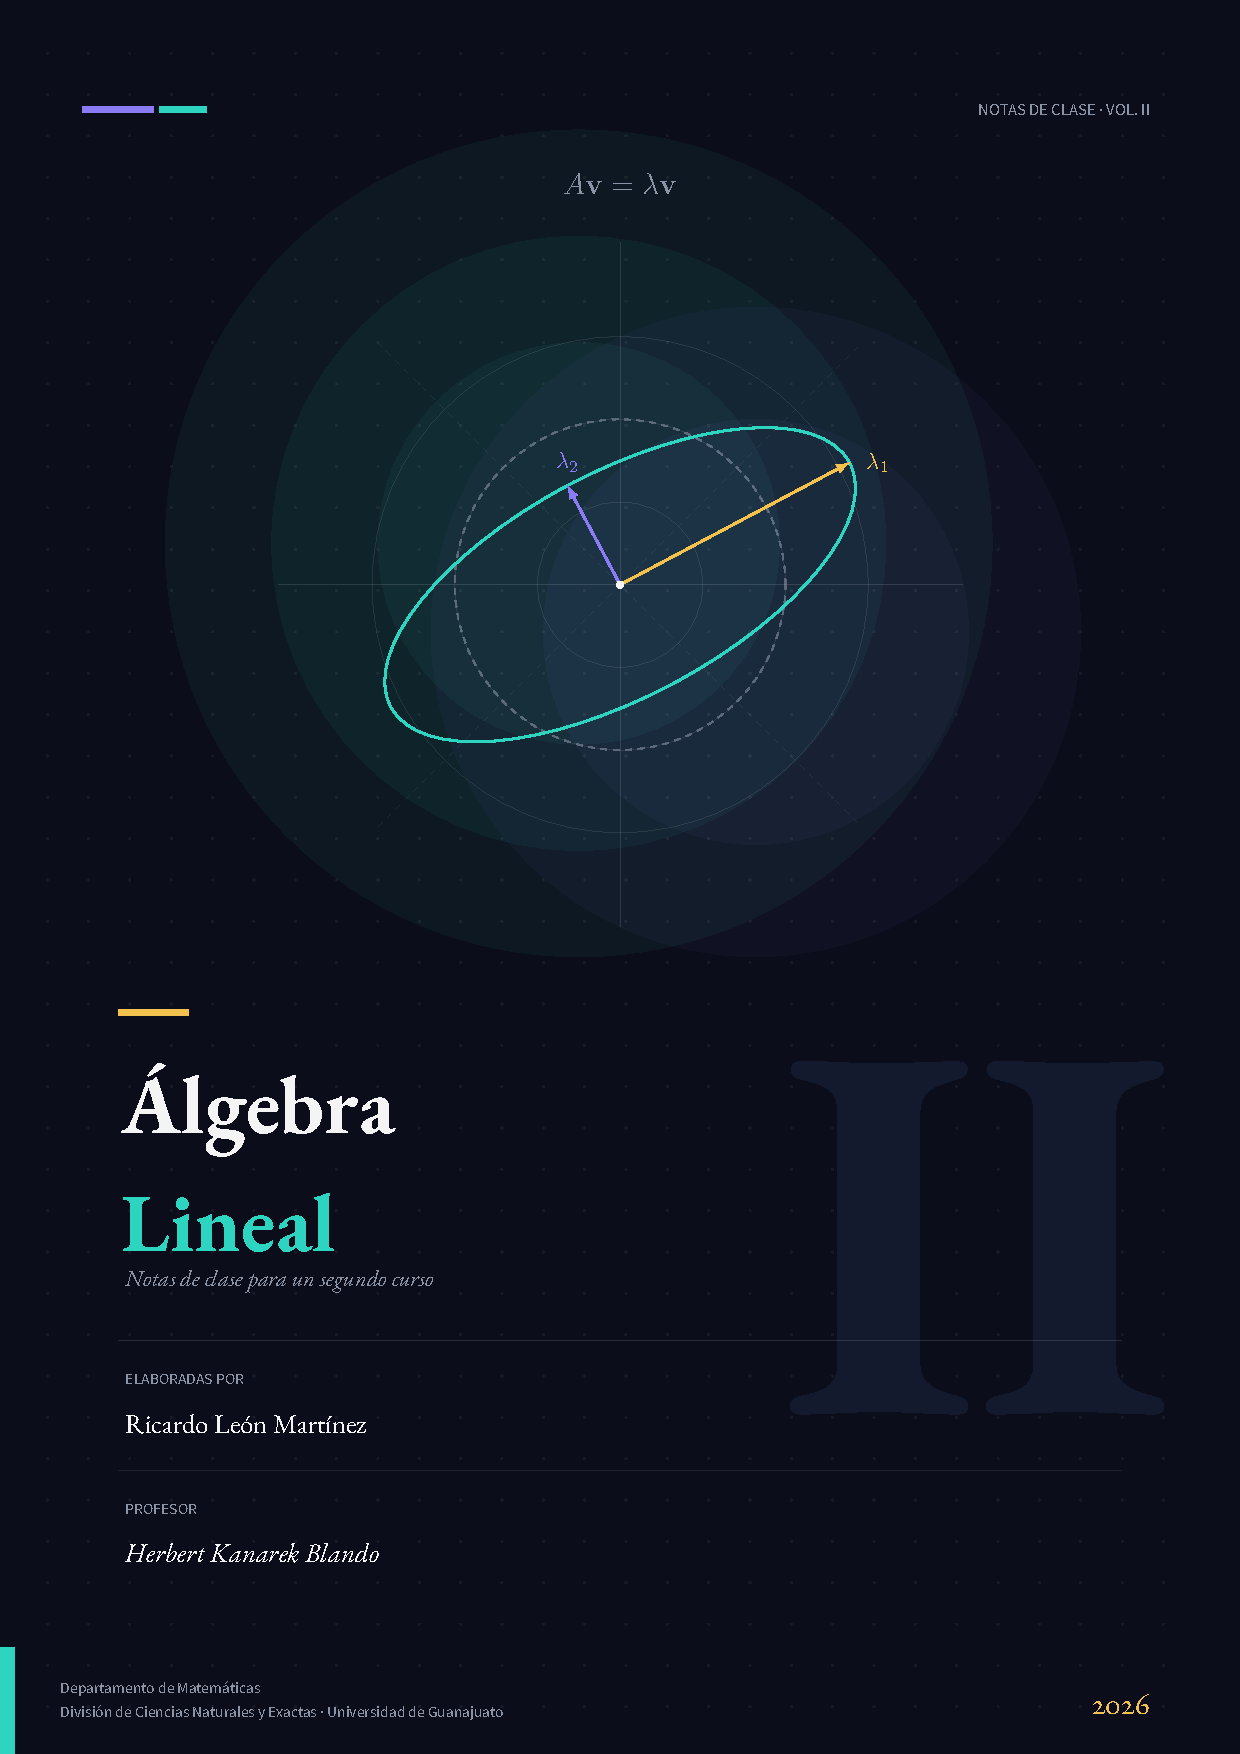
\includepdf[pages=1]{Portada/portada-algebra-lineal-ii.pdf}

    \begin{flushright}
      \thispagestyle{empty}

        \textbf{Ricardo}\\[0.3cm]
        \textit{A los tacos el paisa 2\\
        porque son unos rifados.\\
        A Román porque sufrió redactando\\
        estas notas.\\
        A Uicab por su libreta\\
        de lineal.\\
        Al grupo de todos ínfimos porque\\
        hacen más llevadera la universidad.\\
        Y a Sam, porque aunque no entienda\\
        del todo estas notas,\\
        siempre estuvo ahí.\\
        Y a Kaori, porque entre tareas, estrés\\
        y examenes, también estuvo ahí.}\\[1.2cm]
    \end{flushright}

    % ---------------- NOTA DE ERRORES ----------------

    \cleardoublepage
    \thispagestyle{empty}

    \begin{mdframed}[style=mdgreenbox]
        \begin{center}
        \small
        Estas notas fueron elaboradas con fines académicos.\\
        A pesar del cuidado puesto en su redacción,\\
        es posible que existan errores u omisiones.\\[0.3cm]

        Cualquier corrección, sugerencia o comentario será bienvenido
        en el correo: \\[0.3cm]

        ricardo.leon@cimat.mx
        \end{center}
    \end{mdframed}

    % -------------------------------------------------
    
    \setcounter{page}{1}
    \tableofcontents

    \chapter{Diagonalización}

    Este capítulo trata el problema de la diagonalización. Dado un operador lineal $T$ sobre un espacio vectorial $V$ de dimensión finita, buscamos responder a las siguientes preguntas:

    \begin{enumerate}
        \item ¿Existe una base ordenada $\BB$ de $V$ tal que $[T]_{\BB}$ sea una matriz diagonal?
        \item Si tal base existe, ¿cómo se encuentra?
    \end{enumerate}

    Como los cálculos con matrices diagonales son sencillos, responder afirmativamente a la primera pregunta nos permite entender con claridad cómo actúa $T$ sobre $V$, y responder a la segunda nos permite resolver de forma sencilla muchos problemas que pueden formularse en términos de álgebra lineal.

    Una solución al problema de la diagonalización nos lleva de manera natural a los conceptos de \textbf{valor propio} y \textbf{vector propio}. Además del papel que juegan en el problema de la diagonalización, estos conceptos resultan también útiles en el estudio de operadores que no son diagonalizables.

    \section{Valores propios y vectores propios}

    Consideremos, por ejemplo, la reflexión $T$ de $\R^2$ respecto a la recta $y = 2x$. Tomando como base ordenada $\BB'$ un vector director de la recta y un vector normal a ella, la matriz $[T]_{\BB'}$ resulta diagonal. Esto motiva el siguiente nombre para un operador (o una matriz) que admite una base de este tipo.

    \begin{definicion}[Operador diagonalizable]
        Un operador lineal $T$ sobre un espacio vectorial $V$ de dimensión finita se llama \textbf{diagonalizable} si existe una base ordenada $\BB$ de $V$ tal que $[T]_{\BB}$ es una matriz diagonal. Una matriz cuadrada $A$ se llama \textbf{diagonalizable} si $L_A$ es diagonalizable.
    \end{definicion}

    Queremos determinar cuándo un operador lineal $T$ sobre un espacio vectorial de dimensión finita es diagonalizable y, en caso afirmativo, cómo obtener una base ordenada $\BB = \{v_1, v_2, \dots, v_n\}$ de $V$ tal que $[T]_{\BB}$ sea una matriz diagonal. Observemos que si $D = [T]_{\BB}$ es diagonal, entonces para cada vector $v_j \in \BB$ se tiene
    \begin{equation*}
        T(v_j) = \sum_{i=1}^{n} D_{ij} v_i = D_{jj} v_j = \lambda_j v_j,
    \end{equation*}
    donde $\lambda_j = D_{jj}$.

    Recíprocamente, si $\BB = \{v_1, v_2, \dots, v_n\}$ es una base ordenada de $V$ tal que $T(v_j) = \lambda_j v_j$ para ciertos escalares $\lambda_1, \dots, \lambda_n$, entonces claramente
    \begin{equation*}
        [T]_{\BB} =
        \begin{pmatrix}
            \lambda_1 & 0 & \cdots & 0 \\
            0 & \lambda_2 & \cdots & 0 \\
            \vdots & & \ddots & \vdots \\
            0 & 0 & \cdots & \lambda_n
        \end{pmatrix}.
    \end{equation*}

    En el párrafo anterior, cada vector $v$ de la base $\BB$ satisface la condición $T(v) = \lambda v$ para algún escalar $\lambda$; y, por estar en una base, $v$ es no nulo. Estas observaciones motivan las siguientes definiciones.

    \begin{definicion}[Valor propio y vector propio]
        Sea $T$ un operador lineal sobre un espacio vectorial $V$. Un vector $v \in V$ no nulo se llama \textbf{vector propio} de $T$ si existe un escalar $\lambda$ tal que $T(v) = \lambda v$. Al escalar $\lambda$ se le llama \textbf{valor propio} de $T$ correspondiente al vector propio $v$.

        Sea $A \in M_{n \times n}(F)$. Un vector $v \in F^n$ no nulo se llama \textbf{vector propio} de $A$ si $v$ es vector propio de $L_A$; es decir, si $Av = \lambda v$ para algún escalar $\lambda$. Al escalar $\lambda$ se le llama \textbf{valor propio} de $A$ correspondiente al vector propio $v$.
    \end{definicion}

    También se usan los términos \textit{vector característico} y \textit{valor característico} como sinónimos de vector propio y valor propio, respectivamente.

    Notemos que un vector es vector propio de una matriz $A$ si y solo si lo es de $L_A$; análogamente, un escalar $\lambda$ es valor propio de $A$ si y solo si lo es de $L_A$. Con esta terminología, podemos resumir la discusión anterior de la siguiente manera.

    \begin{teorema}
        Un operador lineal $T$ sobre un espacio vectorial $V$ de dimensión finita es diagonalizable si y solo si existe una base ordenada $\BB = \{v_1, v_2, \dots, v_n\}$ de $V$ formada por vectores propios de $T$. Más aún, si $T$ es diagonalizable, $\BB$ es una base de vectores propios de $T$ y $D = [T]_{\BB}$, entonces $D$ es una matriz diagonal y $D_{jj}$ es el valor propio correspondiente a $v_j$, para $1 \leq j \leq n$.
    \end{teorema}

    \begin{proof}
        Es exactamente lo que se probó en los dos párrafos anteriores a la definición de valor y vector propio.
    \end{proof}

    Diagonalizar una matriz o un operador lineal consiste, entonces, en encontrar una base formada por vectores propios y los valores propios correspondientes.

    Antes de continuar con el estudio del problema de diagonalización, veamos tres ejemplos de valores y vectores propios.

    \begin{ejemplo}
        Sean
        \begin{equation*}
            A = \begin{pmatrix} 1 & 3 \\ 4 & 2 \end{pmatrix}, \qquad
            v_1 = \begin{pmatrix} 1 \\ -1 \end{pmatrix}, \qquad
            v_2 = \begin{pmatrix} 3 \\ 4 \end{pmatrix}.
        \end{equation*}
        Como
        \begin{equation*}
            L_A(v_1) = \begin{pmatrix} 1 & 3 \\ 4 & 2 \end{pmatrix}\begin{pmatrix} 1 \\ -1 \end{pmatrix} = \begin{pmatrix} -2 \\ 2 \end{pmatrix} = -2 v_1,
        \end{equation*}
        $v_1$ es vector propio de $L_A$, y por tanto de $A$, con valor propio $\lambda_1 = -2$. Además,
        \begin{equation*}
            L_A(v_2) = \begin{pmatrix} 1 & 3 \\ 4 & 2 \end{pmatrix}\begin{pmatrix} 3 \\ 4 \end{pmatrix} = \begin{pmatrix} 15 \\ 20 \end{pmatrix} = 5 v_2,
        \end{equation*}
        así que $v_2$ es vector propio de $L_A$, y de $A$, con valor propio $\lambda_2 = 5$. Notemos que $\BB = \{v_1, v_2\}$ es una base ordenada de $\R^2$ formada por vectores propios de $A$ y de $L_A$, por lo que $A$ y $L_A$ son diagonalizables. Más aún, por el teorema anterior,
        \begin{equation*}
            [L_A]_{\BB} = \begin{pmatrix} -2 & 0 \\ 0 & 5 \end{pmatrix}.
        \end{equation*}
    \end{ejemplo}

    \begin{ejemplo}
        Sea $T$ el operador lineal sobre $\R^2$ que gira cada vector del plano un ángulo de $\pi/2$. Geométricamente es claro que, para cualquier vector no nulo $v$, los vectores $v$ y $T(v)$ no son colineales; por tanto $T(v)$ no es múltiplo de $v$. Así, $T$ no tiene vectores propios ni, en consecuencia, valores propios. Existen entonces operadores (y matrices) sin valores propios ni vectores propios; en particular, no son diagonalizables.
    \end{ejemplo}

    \begin{ejemplo}
        Sea $C^\infty(\R)$ el conjunto de las funciones $f : \R \to \R$ que tienen derivadas de todos los órdenes. (Así, $C^\infty(\R)$ contiene a los polinomios, las funciones seno y coseno, las funciones exponenciales, etc.) Claramente $C^\infty(\R)$ es un subespacio del espacio vectorial $\mathcal{F}(\R,\R)$ de todas las funciones de $\R$ en $\R$. Sea $T : C^\infty(\R) \to C^\infty(\R)$ dada por $T(f) = f'$, la derivada de $f$. Es fácil verificar que $T$ es un operador lineal sobre $C^\infty(\R)$. Determinemos los valores y vectores propios de $T$.

        Supongamos que $f$ es un vector propio de $T$ con valor propio correspondiente $\lambda$. Entonces $f' = T(f) = \lambda f$, una ecuación diferencial de primer orden cuyas soluciones son de la forma $f(t) = c e^{\lambda t}$ para alguna constante $c$. En consecuencia, todo número real $\lambda$ es valor propio de $T$, y a él corresponden los vectores propios de la forma $c e^{\lambda t}$ con $c \neq 0$. En particular, para $\lambda = 0$ los vectores propios son las funciones constantes no nulas.
    \end{ejemplo}

    Para obtener una base de vectores propios de una matriz (o de un operador lineal), necesitamos primero poder determinar sus valores y vectores propios. El siguiente teorema da un método para calcular los valores propios.

    \begin{teorema}
        Sea $A \in M_{n \times n}(F)$. Un escalar $\lambda$ es valor propio de $A$ si y solo si $\det(A - \lambda I_n) = 0$.
    \end{teorema}

    \begin{proof}
        Un escalar $\lambda$ es valor propio de $A$ si y solo si existe $v \in F^n$ no nulo tal que $Av = \lambda v$, es decir, tal que $(A - \lambda I_n)v = 0$; equivalentemente, si y solo si $\ker(A - \lambda I_n) \neq \{0\}$. Como una matriz cuadrada $B$ no es invertible si y solo si existe $v \neq 0$ con $Bv = 0$, lo anterior ocurre si y solo si $A - \lambda I_n$ no es invertible, lo cual a su vez equivale a $\det(A - \lambda I_n) = 0$.
    \end{proof}

    \begin{definicion}[Polinomio característico]
        Sea $A \in M_{n \times n}(F)$. Al polinomio $f(t) = \det(A - tI_n)$ se le llama \textbf{polinomio característico} de $A$.
    \end{definicion}

    El teorema anterior dice que los valores propios de una matriz son los ceros de su polinomio característico. Para determinar los valores propios de una matriz o de un operador lineal, normalmente se calcula su polinomio característico, como en el siguiente ejemplo.

    \begin{ejemplo}
        Para encontrar los valores propios de
        \begin{equation*}
            A = \begin{pmatrix} 1 & 1 \\ 4 & 1 \end{pmatrix} \in M_{2\times 2}(\R),
        \end{equation*}
        calculamos su polinomio característico:
        \begin{equation*}
            \det(A - tI_2) = \det\begin{pmatrix} 1 - t & 1 \\ 4 & 1 - t \end{pmatrix} = t^2 - 2t - 3 = (t-3)(t+1).
        \end{equation*}
        Por el teorema anterior, los únicos valores propios de $A$ son $3$ y $-1$.
    \end{ejemplo}

    Se prueba fácilmente que matrices semejantes tienen el mismo polinomio característico: si $B = P^{-1}AP$ para alguna matriz invertible $P$, entonces
    \begin{equation*}
        \det(B - tI_n) = \det\left(P^{-1}(A-tI_n)P\right) = \det(P^{-1})\det(A-tI_n)\det(P) = \det(A - tI_n).
    \end{equation*}
    Este hecho nos permite definir el polinomio característico de un operador lineal de la siguiente manera.

    \begin{definicion}[Polinomio característico de un operador]
        Sea $T$ un operador lineal sobre un espacio vectorial $V$ de dimensión finita $n$, y sea $\BB$ una base ordenada de $V$. Se define el \textbf{polinomio característico} $f(t)$ de $T$ como el polinomio característico de $A = [T]_{\BB}$, es decir,
        \begin{equation*}
            f(t) = \det(A - tI_n).
        \end{equation*}
    \end{definicion}

    La observación anterior muestra que esta definición no depende de la base ordenada $\BB$ elegida. Así, si $T$ es un operador lineal sobre un espacio vectorial $V$ de dimensión finita y $\BB$ es una base ordenada de $V$, entonces $\lambda$ es valor propio de $T$ si y solo si lo es de $[T]_{\BB}$. Con frecuencia denotamos el polinomio característico de un operador $T$ por $\det(T - tI)$.

    \begin{ejemplo}
        Sea $T$ el operador lineal sobre $P_2(\R)$ dado por $T(f(x)) = f(x) + (x+1)f'(x)$, sea $\BB$ la base canónica de $P_2(\R)$, y sea $A = [T]_{\BB}$. Entonces
        \begin{equation*}
            A = \begin{pmatrix} 1 & 1 & 0 \\ 0 & 2 & 2 \\ 0 & 0 & 3 \end{pmatrix}.
        \end{equation*}
        El polinomio característico de $T$ es
        \begin{align*}
            \det(A - tI_3) &= \det\begin{pmatrix} 1-t & 1 & 0 \\ 0 & 2-t & 2 \\ 0 & 0 & 3-t \end{pmatrix} \\
            &= (1-t)(2-t)(3-t) \\
            &= -(t-1)(t-2)(t-3).
        \end{align*}
        Así, $\lambda$ es valor propio de $T$ (o de $A$) si y solo si $\lambda = 1, 2$ o $3$.
    \end{ejemplo}

    Los ejemplos anteriores sugieren que el polinomio característico de una matriz $A$ de tamaño $n \times n$ es un polinomio de grado $n$. El siguiente teorema confirma esto y añade más información.

    \begin{teorema}
        Sea $A \in M_{n\times n}(F)$.
        \begin{enumerate}[label=(\alph*)]
            \item El polinomio característico de $A$ tiene grado $n$ y coeficiente principal $(-1)^n$.
            \item $A$ tiene a lo más $n$ valores propios distintos.
        \end{enumerate}
    \end{teorema}

    \begin{proof}
        Probamos (a) por inducción sobre $n$. Para $n=1$, $A = (a_{11})$ y $\det(A - tI_1) = a_{11} - t$, un polinomio de grado $1$ y coeficiente principal $-1 = (-1)^1$.

        Supongamos el resultado válido para matrices de tamaño $(n-1)\times(n-1)$, con $n \geq 2$, y sea $A \in M_{n\times n}(F)$. Desarrollando $\det(A - tI_n)$ por cofactores a lo largo de la primera columna,
        \begin{equation*}
            \det(A - tI_n) = (a_{11} - t)\det(M_{11}) + \sum_{i=2}^{n} (-1)^{i+1} a_{i1} \det(M_{i1}),
        \end{equation*}
        donde $M_{i1}$ es la matriz que se obtiene al eliminar el renglón $i$ y la columna $1$ de $A - tI_n$. Para $i \geq 2$, la variable $t$ aparece en $M_{i1}$ en a lo más $n-2$ entradas de la diagonal, así que $\det(M_{i1})$ es un polinomio en $t$ de grado a lo más $n-2$. Por otro lado, $M_{11}$ es la matriz $(n-1)\times(n-1)$ que se obtiene al eliminar el primer renglón y la primera columna de $A - tI_n$; es decir, $M_{11} = A' - tI_{n-1}$, donde $A'$ es la submatriz correspondiente de $A$. Por hipótesis de inducción, $\det(M_{11})$ es un polinomio en $t$ de grado $n-1$ con coeficiente principal $(-1)^{n-1}$. Así,
        \begin{equation*}
            \det(A - tI_n) = (a_{11}-t)\det(M_{11}) + (\text{términos de grado} \leq n-2),
        \end{equation*}
        que es un polinomio en $t$ de grado $n$, cuyo coeficiente de $t^n$ proviene únicamente de $(-t)\cdot(-1)^{n-1}t^{n-1} = (-1)^n t^n$. Esto prueba (a).

        Para (b), como el polinomio característico de $A$ tiene grado $n$, tiene a lo más $n$ raíces distintas; por el teorema anterior, los valores propios de $A$ son precisamente los ceros de este polinomio, así que $A$ tiene a lo más $n$ valores propios distintos.
    \end{proof}

    El siguiente teorema da un procedimiento para determinar los vectores propios correspondientes a un valor propio dado.

    \begin{teorema}
        Sea $T$ un operador lineal sobre un espacio vectorial $V$, y sea $\lambda$ un valor propio de $T$. Un vector $v \in V$ es vector propio de $T$ correspondiente a $\lambda$ si y solo si $v \neq 0$ y $v \in \ker(T - \lambda I)$.
    \end{teorema}

    \begin{proof}
        Por definición, $v$ es vector propio de $T$ correspondiente a $\lambda$ si y solo si $v \neq 0$ y $T(v) = \lambda v$. Esta última igualdad equivale a $(T-\lambda I)(v) = T(v) - \lambda v = 0$, es decir, a $v \in \ker(T-\lambda I)$. Por lo tanto, $v$ es vector propio de $T$ correspondiente a $\lambda$ si y solo si $v \neq 0$ y $v \in \ker(T-\lambda I)$.
    \end{proof}

    \begin{ejemplo}
        Para encontrar todos los vectores propios de la matriz
        \begin{equation*}
            A = \begin{pmatrix} 1 & 1 \\ 4 & 1 \end{pmatrix},
        \end{equation*}
        recordemos que, en el ejemplo anterior, $A$ tiene dos valores propios, $\lambda_1 = 3$ y $\lambda_2 = -1$. Comencemos por encontrar los vectores propios correspondientes a $\lambda_1 = 3$. Sea
        \begin{equation*}
            B_1 = A - \lambda_1 I = \begin{pmatrix} 1 & 1 \\ 4 & 1 \end{pmatrix} - \begin{pmatrix} 3 & 0 \\ 0 & 3 \end{pmatrix} = \begin{pmatrix} -2 & 1 \\ 4 & -2 \end{pmatrix}.
        \end{equation*}
        Entonces
        \begin{equation*}
            x = \begin{pmatrix} x_1 \\ x_2 \end{pmatrix} \in \R^2
        \end{equation*}
        es vector propio correspondiente a $\lambda_1 = 3$ si y solo si $x \neq 0$ y $x \in \ker(L_{B_1})$; es decir, $x \neq 0$ y
        \begin{equation*}
            \begin{pmatrix} -2 & 1 \\ 4 & -2 \end{pmatrix}\begin{pmatrix} x_1 \\ x_2 \end{pmatrix} = \begin{pmatrix} -2x_1 + x_2 \\ 4x_1 - 2x_2 \end{pmatrix} = \begin{pmatrix} 0 \\ 0 \end{pmatrix}.
        \end{equation*}
        Claramente, el conjunto de todas las soluciones de esta ecuación es
        \begin{equation*}
            \left\{ t\begin{pmatrix} 1 \\ 2 \end{pmatrix} : t \in \R \right\}.
        \end{equation*}
        Así, $x$ es vector propio correspondiente a $\lambda_1 = 3$ si y solo si
        \begin{equation*}
            x = t \begin{pmatrix} 1 \\ 2 \end{pmatrix} \quad \text{para algún } t \neq 0.
        \end{equation*}

        Supongamos ahora que $x$ es vector propio de $A$ correspondiente a $\lambda_2 = -1$. Sea
        \begin{equation*}
            B_2 = A - \lambda_2 I = \begin{pmatrix} 1 & 1 \\ 4 & 1 \end{pmatrix} - \begin{pmatrix} -1 & 0 \\ 0 & -1 \end{pmatrix} = \begin{pmatrix} 2 & 1 \\ 4 & 2 \end{pmatrix}.
        \end{equation*}
        Entonces $x = \begin{pmatrix} x_1 \\ x_2 \end{pmatrix} \in \ker(L_{B_2})$ si y solo si $x$ es solución del sistema
        \begin{align*}
            2x_1 + x_2 &= 0 \\
            4x_1 + 2x_2 &= 0.
        \end{align*}
        Por tanto,
        \begin{equation*}
            \ker(L_{B_2}) = \left\{ t\begin{pmatrix} 1 \\ -2 \end{pmatrix} : t \in \R \right\},
        \end{equation*}
        así que $x$ es vector propio correspondiente a $\lambda_2 = -1$ si y solo si
        \begin{equation*}
            x = t \begin{pmatrix} 1 \\ -2 \end{pmatrix} \quad \text{para algún } t \neq 0.
        \end{equation*}

        Observemos que
        \begin{equation*}
            \left\{ \begin{pmatrix} 1 \\ 2 \end{pmatrix}, \begin{pmatrix} 1 \\ -2 \end{pmatrix} \right\}
        \end{equation*}
        es una base de $\R^2$ formada por vectores propios de $A$. Por tanto $L_A$, y en consecuencia $A$, es diagonalizable.
    \end{ejemplo}

    Supongamos que $\BB$ es una base de $F^n$ formada por vectores propios de $A$. Recordemos, de la teoría de cambio de base, que si $Q$ es la matriz $n\times n$ cuyas columnas son los vectores de $\BB$ (en el orden dado), entonces $Q$ es invertible y $Q^{-1}AQ = [L_A]_{\BB}$ es una matriz diagonal. En el ejemplo anterior, por ejemplo, si
    \begin{equation*}
        Q = \begin{pmatrix} 1 & 1 \\ 2 & -2 \end{pmatrix},
    \end{equation*}
    entonces
    \begin{equation*}
        Q^{-1}AQ = \begin{pmatrix} 3 & 0 \\ 0 & -1 \end{pmatrix}.
    \end{equation*}
    Naturalmente, las entradas diagonales de esta matriz son los valores propios de $A$ que corresponden, respectivamente, a las columnas de $Q$.

    Para encontrar los vectores propios de un operador lineal $T$ sobre un espacio vectorial de dimensión finita, elegimos una base ordenada $\BB$ para $V$ y hacemos $A = [T]_{\BB}$. El siguiente diagrama es el caso particular de una construcción más general de cambio de base en la que $V = W$ y $\BB = \mathcal{C}$. Recordemos que, para $v \in V$, $[v]_{\BB}$ denota el vector de coordenadas de $v$ respecto a $\BB$; escribimos $\phi_{\BB}(v) = [v]_{\BB}$ para la función que a cada vector le asigna su vector de coordenadas. Mostramos que $v \in V$ es vector propio de $T$ correspondiente a $\lambda$ si y solo si $\phi_{\BB}(v)$ es vector propio de $A$ correspondiente a $\lambda$.

    \begin{figure}[H]
        \centering
        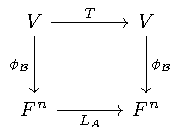
\includegraphics[width=0.3\textwidth]{figuras/diagrama-valores-propios.pdf}
    \end{figure}

    Supongamos que $v$ es vector propio de $T$ correspondiente a $\lambda$. Entonces $T(v) = \lambda v$, de donde
    \begin{equation*}
        A\phi_{\BB}(v) = L_A\phi_{\BB}(v) = \phi_{\BB}T(v) = \phi_{\BB}(\lambda v) = \lambda \phi_{\BB}(v).
    \end{equation*}
    Como $\phi_{\BB}$ es un isomorfismo, $\phi_{\BB}(v) \neq 0$; luego $\phi_{\BB}(v)$ es vector propio de $A$ correspondiente a $\lambda$. Este argumento es reversible, así que también se cumple el recíproco: si $\phi_{\BB}(v)$ es vector propio de $A$ correspondiente a $\lambda$, entonces $v$ es vector propio de $T$ correspondiente a $\lambda$.

    Una formulación equivalente de lo anterior es la siguiente: para un valor propio $\lambda$ de $A$ (y por tanto de $T$), un vector $y \in F^n$ es vector propio de $A$ correspondiente a $\lambda$ si y solo si $\phi_{\BB}^{-1}(y)$ es vector propio de $T$ correspondiente a $\lambda$.

    Hemos reducido así el problema de encontrar los vectores propios de un operador lineal sobre un espacio vectorial de dimensión finita al problema de encontrar los vectores propios de una matriz. El siguiente ejemplo ilustra este procedimiento.

    \begin{ejemplo}
        Sea $T$ el operador lineal sobre $P_2(\R)$ definido en un ejemplo anterior, y sea $\BB$ la base canónica de $P_2(\R)$. Recordemos que $T$ tiene valores propios $1$, $2$ y $3$, y que
        \begin{equation*}
            A = [T]_{\BB} = \begin{pmatrix} 1 & 1 & 0 \\ 0 & 2 & 2 \\ 0 & 0 & 3 \end{pmatrix}.
        \end{equation*}
        Consideramos cada valor propio por separado.

        Sea $\lambda_1 = 1$, y definamos
        \begin{equation*}
            B_1 = A - \lambda_1 I = \begin{pmatrix} 0 & 1 & 0 \\ 0 & 1 & 2 \\ 0 & 0 & 2 \end{pmatrix}.
        \end{equation*}
        Entonces $x = (x_1,x_2,x_3) \in \R^3$ es vector propio correspondiente a $\lambda_1 = 1$ si y solo si $x \neq 0$ y $x$ es solución del sistema
        \begin{align*}
            x_2 &= 0 \\
            x_2 + 2x_3 &= 0 \\
            2x_3 &= 0.
        \end{align*}
        Este sistema tiene tres incógnitas, $x_1, x_2, x_3$, pero $x_1$ no aparece en ninguna ecuación. Como el valor de $x_1$ no afecta al sistema, le asignamos un valor paramétrico $x_1 = a$ y resolvemos para $x_2$ y $x_3$. Claramente $x_2 = x_3 = 0$, de modo que los vectores propios de $A$ correspondientes a $\lambda_1 = 1$ son de la forma
        \begin{equation*}
            a\begin{pmatrix} 1 \\ 0 \\ 0 \end{pmatrix} = a\, e_1
        \end{equation*}
        para $a \neq 0$. En consecuencia, los vectores propios de $T$ correspondientes a $\lambda_1 = 1$ son de la forma
        \begin{equation*}
            \phi_{\BB}^{-1}(a e_1) = a\, \phi_{\BB}^{-1}(e_1) = a \cdot 1 = a
        \end{equation*}
        para cualquier $a \neq 0$. Es decir, los polinomios constantes no nulos son los vectores propios de $T$ correspondientes a $\lambda_1 = 1$.

        Sea ahora $\lambda_2 = 2$, y definamos
        \begin{equation*}
            B_2 = A - \lambda_2 I = \begin{pmatrix} -1 & 1 & 0 \\ 0 & 0 & 2 \\ 0 & 0 & 1 \end{pmatrix}.
        \end{equation*}
        Se verifica fácilmente que
        \begin{equation*}
            \ker(L_{B_2}) = \left\{ a\begin{pmatrix} 1 \\ 1 \\ 0 \end{pmatrix} : a \in \R \right\},
        \end{equation*}
        y por tanto los vectores propios de $T$ correspondientes a $\lambda_2 = 2$ son de la forma
        \begin{equation*}
            \phi_{\BB}^{-1}\left(a\begin{pmatrix} 1\\1\\0\end{pmatrix}\right) = a\, \phi_{\BB}^{-1}(e_1+e_2) = a(1+x)
        \end{equation*}
        para $a \neq 0$.

        Finalmente, consideremos $\lambda_3 = 3$ y
        \begin{equation*}
            B_3 = A - \lambda_3 I = \begin{pmatrix} -2 & 1 & 0 \\ 0 & -1 & 2 \\ 0 & 0 & 0 \end{pmatrix}.
        \end{equation*}
        Como
        \begin{equation*}
            \ker(L_{B_3}) = \left\{ a\begin{pmatrix} 1\\2\\1\end{pmatrix} : a \in \R \right\},
        \end{equation*}
        los vectores propios de $T$ correspondientes a $\lambda_3 = 3$ son de la forma
        \begin{equation*}
            \phi_{\BB}^{-1}\left(a\begin{pmatrix}1\\2\\1\end{pmatrix}\right) = a\,\phi_{\BB}^{-1}(e_1+2e_2+e_3) = a(1+2x+x^2)
        \end{equation*}
        para $a \neq 0$.

        Tomando, para cada valor propio, el vector propio correspondiente con $a=1$, obtenemos $\gamma = \{1,\, 1+x,\, 1+2x+x^2\}$, una base ordenada de $P_2(\R)$ formada por vectores propios de $T$. Así, $T$ es diagonalizable, y
        \begin{equation*}
            [T]_\gamma = \begin{pmatrix} 1 & 0 & 0 \\ 0 & 2 & 0 \\ 0 & 0 & 3 \end{pmatrix}.
        \end{equation*}
    \end{ejemplo}

    Cerramos esta sección con una descripción geométrica de cómo actúa un operador lineal $T$ sobre un vector propio, en el contexto de un espacio vectorial $V$ sobre $\R$. Sea $v$ un vector propio de $T$ y $\lambda$ el valor propio correspondiente. Podemos pensar en $W = \gen{v}$, el subespacio de $V$ de dimensión uno generado por $v$, como una recta en $V$ que pasa por $0$ y por $v$. Para cualquier $w \in W$, $w = cv$ para algún escalar $c$, y por tanto
    \begin{equation*}
        T(w) = T(cv) = cT(v) = c\lambda v = \lambda w;
    \end{equation*}
    así que $T$ actúa sobre los vectores de $W$ multiplicando cada uno por $\lambda$. Existen varias formas en que $T$ puede actuar sobre los vectores de $W$, dependiendo del valor de $\lambda$. Consideramos varios casos (véase la siguiente figura).

    \begin{enumerate}
        \item[\textbf{Caso 1.}] Si $\lambda > 1$, $T$ aleja los vectores de $W$ del origen $0$ por un factor de $\lambda$.
        \item[\textbf{Caso 2.}] Si $\lambda = 1$, $T$ actúa como la identidad sobre $W$.
        \item[\textbf{Caso 3.}] Si $0 < \lambda < 1$, $T$ acerca los vectores de $W$ al origen $0$ por un factor de $\lambda$.
        \item[\textbf{Caso 4.}] Si $\lambda = 0$, $T$ actúa como la transformación cero sobre $W$.
        \item[\textbf{Caso 5.}] Si $\lambda < 0$, $T$ invierte la orientación de $W$; es decir, $T$ manda los vectores de $W$ de un lado de $0$ al otro.
    \end{enumerate}

    \begin{figure}[H]
        \centering
        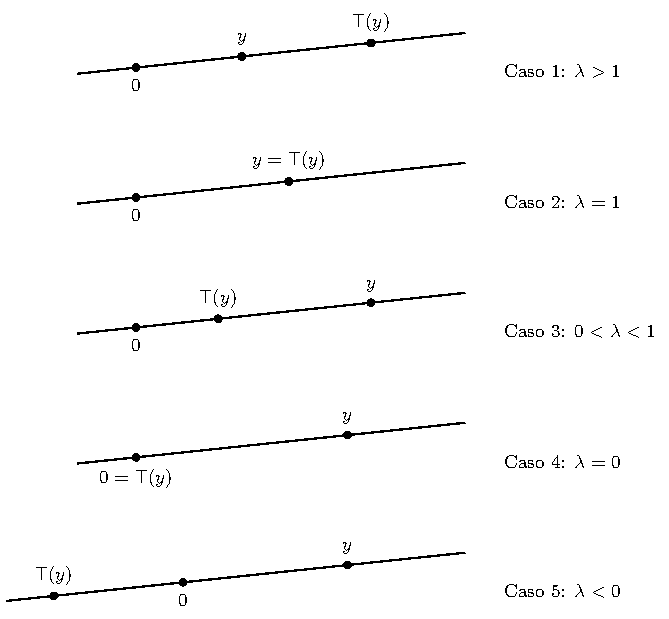
\includegraphics[width=0.55\textwidth]{figuras/accion-vector-propio.pdf}
    \end{figure}

    Para ilustrar estas ideas, consideramos los operadores lineales de los ejemplos anteriores de esta sección.

    Para el operador $T$ sobre $\R^2$ dado por $T(a_1,a_2) = (a_1,-a_2)$ (la reflexión respecto al eje $x$), $e_1$ y $e_2$ son vectores propios de $T$ con valores propios correspondientes $1$ y $-1$, respectivamente. Como $e_1$ y $e_2$ generan al eje $x$ y al eje $y$, respectivamente, $T$ actúa como la identidad sobre el eje $x$ e invierte la orientación del eje $y$.

    Para el operador $T$ sobre $\R^2$ dado por $T(a_1,a_2)=(a_1,0)$ (la proyección sobre el eje $x$), $e_1$ y $e_2$ son vectores propios de $T$ con valores propios correspondientes $1$ y $0$, respectivamente. Así, $T$ actúa como la identidad sobre el eje $x$ y como la transformación cero sobre el eje $y$.

    Por último, generalizamos el ejemplo de la rotación por $\pi/2$ considerando el operador que gira el plano un ángulo $\theta$, definido por
    \begin{equation*}
        T_\theta(a_1,a_2) = (a_1\cos\theta - a_2\sin\theta,\; a_1\sin\theta + a_2\cos\theta).
    \end{equation*}
    Supongamos que $0 < \theta < \pi$. Entonces, para cualquier vector no nulo $v$, los vectores $v$ y $T_\theta(v)$ no son colineales, así que $T_\theta$ no manda ningún subespacio de dimensión uno de $\R^2$ en sí mismo. Por tanto $T_\theta$ no tiene vectores propios y, en consecuencia, tampoco valores propios. Para confirmar esta conclusión, notemos que el polinomio característico de $T_\theta$ es
    \begin{equation*}
        \det(T_\theta - tI) = \det\begin{pmatrix} \cos\theta - t & -\sin\theta \\ \sin\theta & \cos\theta - t\end{pmatrix} = t^2 - (2\cos\theta) t + 1,
    \end{equation*}
    el cual no tiene raíces reales, pues para $0 < \theta < \pi$ el discriminante $4\cos^2\theta - 4$ es negativo.

    \section{Diagonalizabilidad}

    En la sección anterior presentamos el problema de la diagonalización y observamos que no todos los operadores lineales o matrices son diagonalizables. Aunque somos capaces de diagonalizar operadores y matrices, e incluso obtuvimos una condición necesaria y suficiente para la diagonalizabilidad (Teorema~1.1), aún no hemos resuelto el problema de la diagonalización. Lo que falta es una prueba sencilla para determinar si un operador o una matriz puede diagonalizarse, así como un método para encontrar efectivamente una base de vectores propios. En esta sección desarrollamos tal prueba y tal método.

    En el ejemplo de la sección anterior donde diagonalizamos la matriz $\begin{pmatrix}1&1\\4&1\end{pmatrix}$, obtuvimos una base de vectores propios eligiendo un vector propio correspondiente a cada valor propio. En general, este procedimiento no produce una base, pero el siguiente teorema muestra que todo conjunto construido de esta manera es linealmente independiente.

    \begin{teorema}
        Sea $T$ un operador lineal sobre un espacio vectorial $V$, y sean $\lambda_1, \lambda_2, \dots, \lambda_k$ valores propios distintos de $T$. Si $v_1, v_2, \dots, v_k$ son vectores propios de $T$ tales que $\lambda_i$ corresponde a $v_i$ ($1\le i\le k$), entonces $\{v_1,\dots,v_k\}$ es linealmente independiente.
    \end{teorema}

    \begin{proof}
        Procedemos por inducción sobre $k$. Si $k=1$, entonces $v_1\neq 0$ por ser vector propio, y por tanto $\{v_1\}$ es linealmente independiente.

        Supongamos que el teorema es válido para $k-1$ valores propios distintos, con $k-1\geq 1$, y que tenemos $k$ vectores propios $v_1,\dots,v_k$ correspondientes a los valores propios distintos $\lambda_1,\dots,\lambda_k$. Queremos mostrar que $\{v_1,\dots,v_k\}$ es linealmente independiente. Supongamos que $a_1,\dots,a_k$ son escalares tales que
        \begin{equation*}
            a_1v_1+a_2v_2+\cdots+a_kv_k=0. \tag{$*$}
        \end{equation*}
        Aplicando $T-\lambda_k I$ a ambos lados de ($*$),
        \begin{equation*}
            a_1(\lambda_1-\lambda_k)v_1+a_2(\lambda_2-\lambda_k)v_2+\cdots+a_{k-1}(\lambda_{k-1}-\lambda_k)v_{k-1}=0.
        \end{equation*}
        Por hipótesis de inducción, $\{v_1,\dots,v_{k-1}\}$ es linealmente independiente, así que
        \begin{equation*}
            a_1(\lambda_1-\lambda_k)=a_2(\lambda_2-\lambda_k)=\cdots=a_{k-1}(\lambda_{k-1}-\lambda_k)=0.
        \end{equation*}
        Como $\lambda_1,\dots,\lambda_k$ son distintos, $\lambda_i-\lambda_k\neq 0$ para $1\leq i\leq k-1$, de donde $a_1=a_2=\cdots=a_{k-1}=0$, y ($*$) se reduce a $a_kv_k=0$. Pero $v_k\neq 0$, así que $a_k=0$. En consecuencia $a_1=\cdots=a_k=0$, y $\{v_1,\dots,v_k\}$ es linealmente independiente.
    \end{proof}

    \begin{corolario}
        Sea $T$ un operador lineal sobre un espacio vectorial $V$ de dimensión $n$. Si $T$ tiene $n$ valores propios distintos, entonces $T$ es diagonalizable.
    \end{corolario}

    \begin{proof}
        Supongamos que $T$ tiene $n$ valores propios distintos $\lambda_1,\dots,\lambda_n$. Para cada $i$, elijamos un vector propio $v_i$ correspondiente a $\lambda_i$. Por el teorema anterior, $\{v_1,\dots,v_n\}$ es linealmente independiente, y como $\dim(V)=n$, este conjunto es una base de $V$. Así, por el Teorema~1.1, $T$ es diagonalizable.
    \end{proof}

    \begin{ejemplo}
        Sea
        \begin{equation*}
            A=\begin{pmatrix}1&1\\1&1\end{pmatrix}\in M_{2\times2}(\R).
        \end{equation*}
        El polinomio característico de $A$ (y por tanto de $L_A$) es
        \begin{equation*}
            \det(A-tI)=\det\begin{pmatrix}1-t&1\\1&1-t\end{pmatrix}=t(t-2),
        \end{equation*}
        así que los valores propios de $L_A$ son $0$ y $2$. Como $L_A$ es un operador lineal sobre el espacio vectorial de dimensión dos $\R^2$, concluimos por el corolario anterior que $L_A$ (y por tanto $A$) es diagonalizable.
    \end{ejemplo}

    El recíproco del teorema anterior es falso: no es cierto que, si $T$ es diagonalizable, entonces $T$ tiene $n$ valores propios distintos. Por ejemplo, el operador identidad es diagonalizable aunque tiene un único valor propio, $\lambda=1$.

    Hemos visto que la diagonalizabilidad requiere la existencia de valores propios. De hecho, la diagonalizabilidad impone una condición más fuerte sobre el polinomio característico.

    \begin{definicion}[Polinomio que se escinde]
        Un polinomio $f(t) \in P(F)$ \textbf{se escinde} sobre $F$ si existen escalares $c,a_1,\dots,a_n \in F$ (no necesariamente distintos) tales que
        \begin{equation*}
            f(t)=c(t-a_1)(t-a_2)\cdots(t-a_n).
        \end{equation*}
    \end{definicion}

    Por ejemplo, $t^2-1=(t+1)(t-1)$ se escinde sobre $\R$, pero $(t^2+1)(t-2)$ no se escinde sobre $\R$ porque $t^2+1$ no puede factorizarse como producto de factores lineales sobre $\R$. Sin embargo, $(t^2+1)(t-2)$ sí se escinde sobre $\C$, pues se factoriza como $(t+i)(t-i)(t-2)$. Si $f(t)$ es el polinomio característico de un operador lineal o de una matriz sobre un campo $F$, la afirmación de que $f(t)$ se escinde se entiende como que se escinde sobre $F$.

    \begin{teorema}
        El polinomio característico de todo operador lineal diagonalizable se escinde.
    \end{teorema}

    \begin{proof}
        Sea $T$ un operador lineal diagonalizable sobre el espacio vectorial $V$ de dimensión $n$, y sea $\BB$ una base ordenada de $V$ tal que $[T]_{\BB}=D$ es una matriz diagonal. Supongamos
        \begin{equation*}
            D=\begin{pmatrix}\lambda_1&0&\cdots&0\\0&\lambda_2&\cdots&0\\\vdots&&&\vdots\\0&0&\cdots&\lambda_n\end{pmatrix},
        \end{equation*}
        y sea $f(t)$ el polinomio característico de $T$. Entonces
        \begin{align*}
            f(t)&=\det(D-tI)\\
            &=\det\begin{pmatrix}\lambda_1-t&0&\cdots&0\\0&\lambda_2-t&\cdots&0\\\vdots&&&\vdots\\0&0&\cdots&\lambda_n-t\end{pmatrix}\\
            &=(\lambda_1-t)(\lambda_2-t)\cdots(\lambda_n-t)\\
            &=(-1)^n(t-\lambda_1)(t-\lambda_2)\cdots(t-\lambda_n).
        \end{align*}
        Por lo tanto $f(t)$ se escinde.
    \end{proof}

    De este teorema es claro que, si $T$ es un operador lineal diagonalizable sobre un espacio vectorial de dimensión $n$ que no tiene $n$ valores propios distintos, entonces el polinomio característico de $T$ debe tener ceros repetidos.

    El recíproco del teorema anterior es falso: es decir, el polinomio característico de $T$ puede escindirse sin que $T$ sea diagonalizable (véase el ejemplo que sigue a la definición de subespacio propio, más adelante en esta sección). El siguiente concepto nos ayuda a determinar cuándo un operador cuyo polinomio característico se escinde es diagonalizable.

    \begin{definicion}[Multiplicidad algebraica]
        Sea $\lambda$ un valor propio de un operador lineal o de una matriz, con polinomio característico $f(t)$. La \textbf{multiplicidad algebraica} de $\lambda$ es el mayor entero positivo $k$ tal que $(t-\lambda)^k$ es un factor de $f(t)$.
    \end{definicion}

    \begin{ejemplo}
        Sea
        \begin{equation*}
            A=\begin{pmatrix}3&1&0\\0&3&4\\0&0&4\end{pmatrix},
        \end{equation*}
        cuyo polinomio característico es $f(t)=-(t-3)^2(t-4)$. Así, $\lambda=3$ es valor propio de $A$ con multiplicidad $2$, y $\lambda=4$ es valor propio de $A$ con multiplicidad $1$.
    \end{ejemplo}

    Si $T$ es un operador lineal diagonalizable sobre un espacio vectorial $V$ de dimensión finita, entonces existe una base ordenada $\BB$ de $V$ formada por vectores propios de $T$. Sabemos, por el Teorema~1.1, que $[T]_{\BB}$ es una matriz diagonal cuyas entradas diagonales son los valores propios de $T$. Como el polinomio característico de $T$ es $\det([T]_{\BB}-tI)$, se ve fácilmente que cada valor propio de $T$ debe aparecer como entrada diagonal de $[T]_{\BB}$ exactamente tantas veces como su multiplicidad. Por tanto $\BB$ contiene tantos vectores propios (linealmente independientes) correspondientes a un valor propio dado como la multiplicidad de ese valor propio. Así, el número de vectores propios linealmente independientes correspondientes a un valor propio dado resulta de interés para determinar si un operador puede diagonalizarse. Recordando, del Teorema~1.4, que los vectores propios de $T$ correspondientes al valor propio $\lambda$ son los vectores no nulos del espacio nulo de $T-\lambda I$, estudiamos a continuación este conjunto.

    \begin{definicion}[Subespacio propio]
        Sea $T$ un operador lineal sobre un espacio vectorial $V$, y sea $\lambda$ un valor propio de $T$. Se define
        \begin{equation*}
            E_\lambda=\{x\in V: T(x)=\lambda x\}=\ker(T-\lambda I_V).
        \end{equation*}
        Al conjunto $E_\lambda$ se le llama \textbf{subespacio propio} de $T$ correspondiente al valor propio $\lambda$. Análogamente, se define el subespacio propio de una matriz cuadrada $A$ como el subespacio propio de $L_A$.
    \end{definicion}

    Claramente, $E_\lambda$ es un subespacio de $V$ que consiste del vector cero y de los vectores propios de $T$ correspondientes al valor propio $\lambda$. El número máximo de vectores propios de $T$ linealmente independientes correspondientes a $\lambda$ es, por tanto, la dimensión de $E_\lambda$. El siguiente resultado relaciona esta dimensión con la multiplicidad de $\lambda$.

    \begin{teorema}
        Sea $T$ un operador lineal sobre un espacio vectorial $V$ de dimensión finita, y sea $\lambda$ un valor propio de $T$ de multiplicidad $m$. Entonces $1\leq \dim(E_\lambda)\leq m$.
    \end{teorema}

    \begin{proof}
        Elijamos una base ordenada $\{v_1,\dots,v_p\}$ para $E_\lambda$, extendámosla a una base ordenada $\BB=\{v_1,\dots,v_p,v_{p+1},\dots,v_n\}$ de $V$, y sea $A=[T]_{\BB}$. Como $v_i$ ($1\leq i\leq p$) es vector propio de $T$ correspondiente a $\lambda$,
        \begin{equation*}
            A=\begin{pmatrix}\lambda I_p&B\\O&C\end{pmatrix}
        \end{equation*}
        para ciertas matrices $B$ y $C$. Usando que el determinante de una matriz triangular por bloques es el producto de los determinantes de los bloques diagonales, el polinomio característico de $T$ es
        \begin{align*}
            f(t)&=\det(A-tI_n)=\det\begin{pmatrix}(\lambda-t)I_p&B\\O&C-tI_{n-p}\end{pmatrix}\\
            &=\det((\lambda-t)I_p)\det(C-tI_{n-p})\\
            &=(\lambda-t)^p g(t),
        \end{align*}
        donde $g(t)$ es un polinomio. Así, $(\lambda-t)^p$ es un factor de $f(t)$, y por tanto la multiplicidad de $\lambda$ es al menos $p$, es decir, $p\leq m$. Pero $\dim(E_\lambda)=p$, así que $\dim(E_\lambda)\leq m$. Como $\lambda$ es valor propio, $E_\lambda\neq\{0\}$, de donde $p\geq 1$ y por tanto $\dim(E_\lambda)\geq 1$.
    \end{proof}

    \begin{ejemplo}
        Sea $T$ el operador lineal sobre $P_2(\R)$ definido por $T(f(x))=f'(x)$. La representación matricial de $T$ respecto a la base canónica $\BB$ de $P_2(\R)$ es
        \begin{equation*}
            [T]_{\BB}=\begin{pmatrix}0&1&0\\0&0&2\\0&0&0\end{pmatrix}.
        \end{equation*}
        En consecuencia, el polinomio característico de $T$ es
        \begin{equation*}
            \det([T]_{\BB}-tI)=\det\begin{pmatrix}-t&1&0\\0&-t&2\\0&0&-t\end{pmatrix}=-t^3.
        \end{equation*}
        Así, $T$ tiene un único valor propio, $\lambda=0$, con multiplicidad $3$. Resolviendo $T(f(x))=f'(x)=0$ vemos que $E_\lambda=\ker(T-\lambda I)=\ker(T)$ es el subespacio de $P_2(\R)$ formado por los polinomios constantes. Así, $\{1\}$ es una base de $E_\lambda$, y por tanto $\dim(E_\lambda)=1$. En consecuencia, no existe base de $P_2(\R)$ formada por vectores propios de $T$, y por tanto $T$ no es diagonalizable, aunque su polinomio característico se escinde. Esto muestra que el recíproco del Teorema~1.6 es falso.
    \end{ejemplo}

    \begin{ejemplo}
        Sea $T$ el operador lineal sobre $\R^3$ definido por
        \begin{equation*}
            T\begin{pmatrix}a_1\\a_2\\a_3\end{pmatrix}=\begin{pmatrix}4a_1+a_3\\2a_1+3a_2+2a_3\\a_1+4a_3\end{pmatrix}.
        \end{equation*}
        Determinamos el subespacio propio de $T$ correspondiente a cada valor propio. Sea $\BB$ la base canónica de $\R^3$. Entonces
        \begin{equation*}
            [T]_{\BB}=\begin{pmatrix}4&0&1\\2&3&2\\1&0&4\end{pmatrix},
        \end{equation*}
        y por tanto el polinomio característico de $T$ es
        \begin{equation*}
            \det([T]_{\BB}-tI)=\det\begin{pmatrix}4-t&0&1\\2&3-t&2\\1&0&4-t\end{pmatrix}=-(t-5)(t-3)^2.
        \end{equation*}
        Así, los valores propios de $T$ son $\lambda_1=5$ y $\lambda_2=3$, con multiplicidades $1$ y $2$, respectivamente.

        Como
        \begin{equation*}
            E_{\lambda_1}=\ker(T-\lambda_1 I)=\left\{\begin{pmatrix}x_1\\x_2\\x_3\end{pmatrix}\in\R^3: \begin{pmatrix}-1&0&1\\2&-2&2\\1&0&-1\end{pmatrix}\begin{pmatrix}x_1\\x_2\\x_3\end{pmatrix}=\begin{pmatrix}0\\0\\0\end{pmatrix}\right\},
        \end{equation*}
        $E_{\lambda_1}$ es el espacio solución del sistema
        \begin{align*}
            -x_1&&+\,x_3&=0\\
            2x_1-2x_2&&+2x_3&=0\\
            x_1&&-\,x_3&=0.
        \end{align*}
        Se verifica fácilmente que
        \begin{equation*}
            \left\{\begin{pmatrix}1\\2\\1\end{pmatrix}\right\}
        \end{equation*}
        es una base de $E_{\lambda_1}$. Por tanto $\dim(E_{\lambda_1})=1$.

        Análogamente, $E_{\lambda_2}=\ker(T-\lambda_2 I)$ es el espacio solución del sistema
        \begin{align*}
            x_1&&+\,x_3&=0\\
            2x_1&&+2x_3&=0\\
            x_1&&+\,x_3&=0.
        \end{align*}
        Como la incógnita $x_2$ no aparece en este sistema, le asignamos un valor paramétrico $x_2=s$, e introducimos otro parámetro $t$ para resolver el sistema en $x_1$ y $x_3$. La solución general del sistema es
        \begin{equation*}
            \begin{pmatrix}x_1\\x_2\\x_3\end{pmatrix}=s\begin{pmatrix}0\\1\\0\end{pmatrix}+t\begin{pmatrix}-1\\0\\1\end{pmatrix}, \quad \text{para } s,t\in\R.
        \end{equation*}
        Se sigue que
        \begin{equation*}
            \left\{\begin{pmatrix}0\\1\\0\end{pmatrix}, \begin{pmatrix}-1\\0\\1\end{pmatrix}\right\}
        \end{equation*}
        es una base de $E_{\lambda_2}$, y por tanto $\dim(E_{\lambda_2})=2$.

        En este caso, la multiplicidad de cada valor propio $\lambda_i$ es igual a la dimensión del subespacio propio correspondiente $E_{\lambda_i}$. Observemos que la unión de las dos bases recién obtenidas,
        \begin{equation*}
            \left\{\begin{pmatrix}1\\2\\1\end{pmatrix}, \begin{pmatrix}0\\1\\0\end{pmatrix}, \begin{pmatrix}-1\\0\\1\end{pmatrix}\right\},
        \end{equation*}
        es linealmente independiente y, por tanto, es una base de $\R^3$ formada por vectores propios de $T$. En consecuencia, $T$ es diagonalizable.
    \end{ejemplo}

    Los ejemplos anteriores sugieren que un operador cuyo polinomio característico se escinde es diagonalizable si y solo si, para cada valor propio, la dimensión del subespacio propio correspondiente coincide con su multiplicidad. Esto es, en efecto, cierto, como mostramos a continuación. Comenzamos con el siguiente lema, una ligera variación del Teorema~1.5.

    \begin{lema}
        Sea $T$ un operador lineal, y sean $\lambda_1,\dots,\lambda_k$ valores propios distintos de $T$. Para cada $i=1,\dots,k$, sea $v_i\in E_{\lambda_i}$, el subespacio propio correspondiente a $\lambda_i$. Si
        \begin{equation*}
            v_1+v_2+\cdots+v_k=0,
        \end{equation*}
        entonces $v_i=0$ para todo $i$.
    \end{lema}

    \begin{proof}
        Supongamos lo contrario. Renumerando si es necesario, supongamos que, para algún $1\leq m\leq k$, $v_i\neq 0$ para $1\leq i\leq m$, y $v_i=0$ para $i>m$. Entonces, para cada $i\leq m$, $v_i$ es un vector propio de $T$ correspondiente a $\lambda_i$, y
        \begin{equation*}
            v_1+v_2+\cdots+v_m=0.
        \end{equation*}
        Pero esto contradice al Teorema~1.5, que afirma que estos $v_i$ son linealmente independientes. Concluimos, por tanto, que $v_i=0$ para todo $i$.
    \end{proof}

    \begin{teorema}
        Sea $T$ un operador lineal sobre un espacio vectorial $V$, y sean $\lambda_1,\dots,\lambda_k$ valores propios distintos de $T$. Para cada $i=1,\dots,k$, sea $S_i$ un subconjunto finito y linealmente independiente del subespacio propio $E_{\lambda_i}$. Entonces $S=S_1\cup S_2\cup\cdots\cup S_k$ es un subconjunto linealmente independiente de $V$.
    \end{teorema}

    \begin{proof}
        Para cada $i$, escribamos $S_i=\{v_{i1},v_{i2},\dots,v_{in_i}\}$, de modo que $S=\{v_{ij}: 1\leq j\leq n_i,\ 1\leq i\leq k\}$. Consideremos escalares $\{a_{ij}\}$ tales que
        \begin{equation*}
            \sum_{i=1}^{k}\sum_{j=1}^{n_i}a_{ij}v_{ij}=0.
        \end{equation*}
        Para cada $i$, sea
        \begin{equation*}
            w_i=\sum_{j=1}^{n_i}a_{ij}v_{ij}.
        \end{equation*}
        Entonces $w_i\in E_{\lambda_i}$ para cada $i$, y $w_1+\cdots+w_k=0$. Por el lema anterior, $w_i=0$ para todo $i$. Pero cada $S_i$ es linealmente independiente, así que $a_{ij}=0$ para todos $i,j$. Concluimos que $S$ es linealmente independiente.
    \end{proof}

    El teorema anterior nos indica cómo construir un conjunto linealmente independiente de vectores propios: basta reunir bases de cada uno de los subespacios propios. El siguiente teorema nos dice cuándo el conjunto resultante es una base de todo el espacio.

    \begin{teorema}
        Sea $T$ un operador lineal sobre un espacio vectorial $V$ de dimensión finita tal que el polinomio característico de $T$ se escinde. Sean $\lambda_1,\dots,\lambda_k$ los valores propios distintos de $T$. Entonces:
        \begin{enumerate}[label=(\alph*)]
            \item $T$ es diagonalizable si y solo si la multiplicidad de $\lambda_i$ es igual a $\dim(E_{\lambda_i})$ para todo $i$.
            \item Si $T$ es diagonalizable y $\mathcal{G}_i$ es una base ordenada de $E_{\lambda_i}$ para cada $i$, entonces $\mathcal{G}=\mathcal{G}_1\cup\mathcal{G}_2\cup\cdots\cup\mathcal{G}_k$ es una base ordenada de $V$ formada por vectores propios de $T$.
        \end{enumerate}
    \end{teorema}

    \begin{proof}
        Para cada $i$, sea $m_i$ la multiplicidad de $\lambda_i$, $d_i=\dim(E_{\lambda_i})$, y $n=\dim(V)$.

        Supongamos primero que $T$ es diagonalizable. Sea $\BB$ una base de $V$ formada por vectores propios de $T$. Para cada $i$, sea $\BB_i=\BB\cap E_{\lambda_i}$ el conjunto de vectores de $\BB$ que son vectores propios correspondientes a $\lambda_i$, y sea $n_i$ el número de vectores en $\BB_i$. Entonces $n_i\leq d_i$ para cada $i$, pues $\BB_i$ es un subconjunto linealmente independiente de un subespacio de dimensión $d_i$; y $d_i\leq m_i$ por el Teorema~1.7. Los $n_i$ suman $n$ porque $\BB$ tiene $n$ vectores; los $m_i$ también suman $n$, pues el grado del polinomio característico de $T$ es igual a la suma de las multiplicidades de los valores propios. Así,
        \begin{equation*}
            n=\sum_{i=1}^{k}n_i\leq\sum_{i=1}^{k}d_i\leq\sum_{i=1}^{k}m_i=n.
        \end{equation*}
        Se sigue que $\sum_{i=1}^{k}(m_i-d_i)=0$. Como $(m_i-d_i)\geq 0$ para todo $i$, concluimos que $m_i=d_i$ para todo $i$.

        Recíprocamente, supongamos que $m_i=d_i$ para todo $i$; probamos simultáneamente que $T$ es diagonalizable y (b). Para cada $i$, sea $\mathcal{G}_i$ una base ordenada de $E_{\lambda_i}$, y sea $\mathcal{G}=\mathcal{G}_1\cup\cdots\cup\mathcal{G}_k$. Por el Teorema~1.8, $\mathcal{G}$ es linealmente independiente. Más aún, como $d_i=m_i$ para todo $i$, $\mathcal{G}$ contiene
        \begin{equation*}
            \sum_{i=1}^{k}d_i=\sum_{i=1}^{k}m_i=n
        \end{equation*}
        vectores. Por lo tanto $\mathcal{G}$ es una base ordenada de $V$ formada por vectores propios de $T$, y concluimos que $T$ es diagonalizable.
    \end{proof}

    Este teorema completa nuestro estudio del problema de diagonalización. Resumimos nuestros resultados.

    \subsection*{Prueba para la diagonalización}

    Sea $T$ un operador lineal sobre un espacio vectorial $V$ de dimensión $n$. Entonces $T$ es diagonalizable si y solo si se cumplen las siguientes dos condiciones:
    \begin{enumerate}
        \item El polinomio característico de $T$ se escinde.
        \item Para cada valor propio $\lambda$ de $T$, la multiplicidad de $\lambda$ es igual a $n-\rg(T-\lambda I)$.
    \end{enumerate}

    Estas mismas condiciones pueden usarse para probar si una matriz cuadrada $A$ es diagonalizable, pues la diagonalizabilidad de $A$ equivale a la de $L_A$.

    Si $T$ es un operador diagonalizable y $\mathcal{G}_1,\dots,\mathcal{G}_k$ son bases ordenadas de los subespacios propios de $T$, entonces la unión $\BB=\mathcal{G}_1\cup\cdots\cup\mathcal{G}_k$ es una base ordenada de $V$ formada por vectores propios de $T$, y por tanto $[T]_{\BB}$ es diagonal.

    Al probar si $T$ es diagonalizable, suele ser más sencillo elegir una base conveniente $\mathcal{A}$ para $V$ y trabajar con $B=[T]_{\mathcal{A}}$. Si el polinomio característico de $B$ se escinde, se usa entonces la condición 2 anterior para verificar si la multiplicidad de cada valor propio \textit{repetido} de $B$ coincide con $n-\rg(B-\lambda I)$. (Por el Teorema~1.7, la condición 2 se cumple automáticamente para los valores propios de multiplicidad uno.) Si esto ocurre, entonces $B$, y por tanto $T$, es diagonalizable.

    Si $T$ es diagonalizable y se desea una base $\BB$ de $V$ formada por vectores propios de $T$, se encuentra primero una base para cada subespacio propio de $B$. La unión de estas bases es una base $\mathcal{G}$ de $F^n$ formada por vectores propios de $B$. Cada vector de $\mathcal{G}$ es el vector de coordenadas, respecto a $\mathcal{A}$, de un vector propio de $T$. El conjunto formado por estos $n$ vectores propios de $T$ es la base $\BB$ buscada.

    Más aún, si $A$ es una matriz diagonalizable de tamaño $n\times n$, podemos usar el hecho de que si $Q$ es la matriz cuyas columnas son los vectores de una base de $F^n$ formada por vectores propios de $A$, entonces $Q$ es invertible y $D=Q^{-1}AQ$ es diagonal, con entradas diagonales los valores propios de $A$ correspondientes a las columnas de $Q$.

    A continuación consideramos algunos ejemplos que ilustran las ideas anteriores.

    \begin{ejemplo}
        Probamos la diagonalizabilidad de la matriz
        \begin{equation*}
            A=\begin{pmatrix}3&1&0\\0&3&0\\0&0&4\end{pmatrix}\in M_{3\times 3}(\R).
        \end{equation*}
        El polinomio característico de $A$ es $\det(A-tI)=-(t-4)(t-3)^2$, el cual se escinde, así que se satisface la condición 1 de la prueba de diagonalización. Además $A$ tiene valores propios $\lambda_1=4$ y $\lambda_2=3$, con multiplicidades $1$ y $2$, respectivamente. Como $\lambda_1$ tiene multiplicidad $1$, la condición 2 se satisface para $\lambda_1$. Basta entonces verificar la condición 2 para $\lambda_2$. Como
        \begin{equation*}
            A-\lambda_2 I=\begin{pmatrix}0&1&0\\0&0&0\\0&0&1\end{pmatrix}
        \end{equation*}
        tiene rango $2$, se tiene $3-\rg(A-\lambda_2 I)=1$, lo cual no coincide con la multiplicidad de $\lambda_2$. Por tanto la condición 2 falla para $\lambda_2$, y $A$ no es diagonalizable.
    \end{ejemplo}

    \begin{ejemplo}
        Sea $T$ el operador lineal sobre $P_2(\R)$ definido por
        \begin{equation*}
            T(f(x))=f(1)+f'(0)x+(f'(0)+f''(0))x^2.
        \end{equation*}
        Probamos primero si $T$ es diagonalizable. Sea $\mathcal{A}$ la base canónica de $P_2(\R)$, y sea $B=[T]_{\mathcal{A}}$. Entonces
        \begin{equation*}
            B=\begin{pmatrix}1&1&1\\0&1&0\\0&1&2\end{pmatrix}.
        \end{equation*}
        El polinomio característico de $B$, y por tanto de $T$, es $-(t-1)^2(t-2)$, el cual se escinde. Así, $B$ tiene valores propios $\lambda_1=1$ y $\lambda_2=2$, con multiplicidades $2$ y $1$, respectivamente. La condición 2 se satisface para $\lambda_2$ porque tiene multiplicidad $1$. Basta entonces verificar la condición 2 para $\lambda_1=1$. Para esto,
        \begin{equation*}
            3-\rg(B-\lambda_1 I)=3-\rg\begin{pmatrix}0&1&1\\0&0&0\\0&1&1\end{pmatrix}=3-1=2,
        \end{equation*}
        que coincide con la multiplicidad de $\lambda_1$. Por lo tanto, $T$ es diagonalizable.

        Encontramos ahora una base ordenada $\mathcal{G}$ de $\R^3$ formada por vectores propios de $B$. Consideramos cada valor propio por separado.

        El subespacio propio correspondiente a $\lambda_1=1$ es
        \begin{equation*}
            E_{\lambda_1}=\left\{\begin{pmatrix}x_1\\x_2\\x_3\end{pmatrix}\in\R^3: \begin{pmatrix}0&1&1\\0&0&0\\0&1&1\end{pmatrix}\begin{pmatrix}x_1\\x_2\\x_3\end{pmatrix}=0\right\},
        \end{equation*}
        el cual es el espacio solución del sistema $x_2+x_3=0$, y tiene como base
        \begin{equation*}
            \mathcal{G}_1=\left\{\begin{pmatrix}1\\0\\0\end{pmatrix}, \begin{pmatrix}0\\-1\\1\end{pmatrix}\right\}.
        \end{equation*}

        El subespacio propio correspondiente a $\lambda_2=2$ es
        \begin{equation*}
            E_{\lambda_2}=\left\{\begin{pmatrix}x_1\\x_2\\x_3\end{pmatrix}\in\R^3: \begin{pmatrix}-1&1&1\\0&-1&0\\0&1&0\end{pmatrix}\begin{pmatrix}x_1\\x_2\\x_3\end{pmatrix}=0\right\},
        \end{equation*}
        el espacio solución del sistema $-x_1+x_2+x_3=0,\ x_2=0$, con base
        \begin{equation*}
            \mathcal{G}_2=\left\{\begin{pmatrix}1\\0\\1\end{pmatrix}\right\}.
        \end{equation*}

        Sea
        \begin{equation*}
            \mathcal{G}=\mathcal{G}_1\cup\mathcal{G}_2=\left\{\begin{pmatrix}1\\0\\0\end{pmatrix}, \begin{pmatrix}0\\-1\\1\end{pmatrix}, \begin{pmatrix}1\\0\\1\end{pmatrix}\right\}.
        \end{equation*}
        Entonces $\mathcal{G}$ es una base ordenada de $\R^3$ formada por vectores propios de $B$.

        Finalmente, observamos que los vectores de $\mathcal{G}$ son los vectores de coordenadas, respecto a $\mathcal{A}$, de los vectores del conjunto
        \begin{equation*}
            \BB=\{1,\ -x+x^2,\ 1+x^2\},
        \end{equation*}
        que es una base ordenada de $P_2(\R)$ formada por vectores propios de $T$. Así,
        \begin{equation*}
            [T]_{\BB}=\begin{pmatrix}1&0&0\\0&1&0\\0&0&2\end{pmatrix}.
        \end{equation*}
    \end{ejemplo}

    El siguiente ejemplo es una aplicación de la diagonalización.

    \begin{ejemplo}
        Sea
        \begin{equation*}
            A=\begin{pmatrix}0&-2\\1&3\end{pmatrix}.
        \end{equation*}
        Mostramos que $A$ es diagonalizable y encontramos una matriz $Q$ de tamaño $2\times2$ tal que $Q^{-1}AQ$ sea diagonal. Después mostramos cómo usar este resultado para calcular $A^n$ para cualquier entero positivo $n$.

        El polinomio característico de $A$ es $(t-1)(t-2)$, así que $A$ tiene dos valores propios distintos, $\lambda_1=1$ y $\lambda_2=2$. Aplicando el corolario al Teorema~1.5 al operador $L_A$, vemos que $A$ es diagonalizable. Más aún,
        \begin{equation*}
            \mathcal{G}_1=\left\{\begin{pmatrix}-2\\1\end{pmatrix}\right\}
            \quad\text{y}\quad
            \mathcal{G}_2=\left\{\begin{pmatrix}-1\\1\end{pmatrix}\right\}
        \end{equation*}
        son bases de los subespacios propios $E_{\lambda_1}$ y $E_{\lambda_2}$, respectivamente. Por tanto
        \begin{equation*}
            \mathcal{G}=\mathcal{G}_1\cup\mathcal{G}_2=\left\{\begin{pmatrix}-2\\1\end{pmatrix}, \begin{pmatrix}-1\\1\end{pmatrix}\right\}
        \end{equation*}
        es una base ordenada de $\R^2$ formada por vectores propios de $A$. Sea
        \begin{equation*}
            Q=\begin{pmatrix}-2&-1\\1&1\end{pmatrix}
        \end{equation*}
        la matriz cuyas columnas son los vectores de $\mathcal{G}$. Entonces, por el hecho enunciado al inicio de esta subsección,
        \begin{equation*}
            D=Q^{-1}AQ=[L_A]_{\mathcal{G}}=\begin{pmatrix}1&0\\0&2\end{pmatrix}.
        \end{equation*}

        Para encontrar $A^n$, con $n$ un entero positivo cualquiera, observemos que $A=QDQ^{-1}$. Por tanto
        \begin{align*}
            A^n&=(QDQ^{-1})^n\\
            &=(QDQ^{-1})(QDQ^{-1})\cdots(QDQ^{-1})\\
            &=QD^nQ^{-1}\\
            &=Q\begin{pmatrix}1^n&0\\0&2^n\end{pmatrix}Q^{-1}\\
            &=\begin{pmatrix}-2&-1\\1&1\end{pmatrix}\begin{pmatrix}1&0\\0&2^n\end{pmatrix}\begin{pmatrix}-1&-1\\1&2\end{pmatrix}\\
            &=\begin{pmatrix}2-2^n&2-2^{n+1}\\-1+2^n&-1+2^{n+1}\end{pmatrix}.
        \end{align*}
    \end{ejemplo}

    \subsection*{Sistemas de ecuaciones diferenciales}

    Consideremos el sistema de ecuaciones diferenciales
    \begin{align*}
        x_1'&=3x_1+x_2+x_3\\
        x_2'&=2x_1+4x_2+2x_3\\
        x_3'&=-x_1-x_2+x_3,
    \end{align*}
    donde, para cada $i$, $x_i=x_i(t)$ es una función real diferenciable de la variable real $t$. Claramente este sistema tiene una solución, a saber, aquella en la que cada $x_i(t)$ es la función cero. Determinamos todas las soluciones de este sistema.

    Sea $x:\R\to\R^3$ la función definida por
    \begin{equation*}
        x(t)=\begin{pmatrix}x_1(t)\\x_2(t)\\x_3(t)\end{pmatrix}.
    \end{equation*}
    La \textbf{derivada} de $x$, denotada $x'$, se define por
    \begin{equation*}
        x'(t)=\begin{pmatrix}x_1'(t)\\x_2'(t)\\x_3'(t)\end{pmatrix}.
    \end{equation*}
    Sea
    \begin{equation*}
        A=\begin{pmatrix}3&1&1\\2&4&2\\-1&-1&1\end{pmatrix}
    \end{equation*}
    la matriz de coeficientes del sistema dado, de modo que podemos reescribir el sistema como la ecuación matricial $x'=Ax$.

    Se puede verificar que, para
    \begin{equation*}
        Q=\begin{pmatrix}-1&0&-1\\0&-1&-2\\1&1&1\end{pmatrix}
        \quad\text{y}\quad
        D=\begin{pmatrix}2&0&0\\0&2&0\\0&0&4\end{pmatrix},
    \end{equation*}
    se tiene $Q^{-1}AQ=D$. Sustituyendo $A=QDQ^{-1}$ en $x'=Ax$ obtenemos $x'=QDQ^{-1}x$, o equivalentemente, $Q^{-1}x'=DQ^{-1}x$. La función $y:\R\to\R^3$ definida por $y(t)=Q^{-1}x(t)$ es diferenciable, y $y'=Q^{-1}x'$. Así, el sistema original puede escribirse como $y'=Dy$.

    Como $D$ es una matriz diagonal, el sistema $y'=Dy$ es fácil de resolver. Escribiendo
    \begin{equation*}
        y(t)=\begin{pmatrix}y_1(t)\\y_2(t)\\y_3(t)\end{pmatrix},
    \end{equation*}
    podemos reescribir $y'=Dy$ como
    \begin{equation*}
        \begin{pmatrix}y_1'(t)\\y_2'(t)\\y_3'(t)\end{pmatrix}=\begin{pmatrix}2&0&0\\0&2&0\\0&0&4\end{pmatrix}\begin{pmatrix}y_1(t)\\y_2(t)\\y_3(t)\end{pmatrix}=\begin{pmatrix}2y_1(t)\\2y_2(t)\\4y_3(t)\end{pmatrix}.
    \end{equation*}
    Las tres ecuaciones
    \begin{align*}
        y_1'&=2y_1\\
        y_2'&=2y_2\\
        y_3'&=4y_3
    \end{align*}
    son independientes entre sí, y por tanto pueden resolverse por separado. Como vimos en un ejemplo de la sección anterior, la solución general de estas ecuaciones es $y_1(t)=c_1e^{2t}$, $y_2(t)=c_2e^{2t}$ y $y_3(t)=c_3e^{4t}$, donde $c_1,c_2,c_3$ son constantes arbitrarias. Finalmente,
    \begin{align*}
        \begin{pmatrix}x_1(t)\\x_2(t)\\x_3(t)\end{pmatrix}=x(t)=Qy(t)&=\begin{pmatrix}-1&0&-1\\0&-1&-2\\1&1&1\end{pmatrix}\begin{pmatrix}c_1e^{2t}\\c_2e^{2t}\\c_3e^{4t}\end{pmatrix}\\
        &=\begin{pmatrix}-c_1e^{2t}-c_3e^{4t}\\-c_2e^{2t}-2c_3e^{4t}\\c_1e^{2t}+c_2e^{2t}+c_3e^{4t}\end{pmatrix}
    \end{align*}
    nos da la solución general del sistema original. Observemos que esta solución puede escribirse como
    \begin{equation*}
        x(t)=e^{2t}\left[c_1\begin{pmatrix}-1\\0\\1\end{pmatrix}+c_2\begin{pmatrix}0\\-1\\1\end{pmatrix}\right]+e^{4t}\left[c_3\begin{pmatrix}-1\\-2\\1\end{pmatrix}\right].
    \end{equation*}
    Las expresiones entre corchetes son vectores arbitrarios de $E_{\lambda_1}$ y $E_{\lambda_2}$, respectivamente, donde $\lambda_1=2$ y $\lambda_2=4$. Así, la solución general del sistema original es $x(t)=e^{2t}z_1+e^{4t}z_2$, donde $z_1\in E_{\lambda_1}$ y $z_2\in E_{\lambda_2}$.

    \subsection*{Sumas directas}

    Sea $T$ un operador lineal sobre un espacio vectorial $V$ de dimensión finita. Existe una manera de descomponer $V$ en subespacios más simples que ofrece información sobre el comportamiento de $T$. Este enfoque es especialmente útil para operadores no diagonalizables. En el caso de operadores diagonalizables, los subespacios más simples son los subespacios propios del operador.

    \begin{definicion}[Suma de subespacios]
        Sean $W_1,W_2,\dots,W_k$ subespacios de un espacio vectorial $V$. Se define la \textbf{suma} de estos subespacios como el conjunto
        \begin{equation*}
            \{v_1+v_2+\cdots+v_k: v_i\in W_i \text{ para } 1\leq i\leq k\},
        \end{equation*}
        el cual se denota por $W_1+W_2+\cdots+W_k$ o $\sum_{i=1}^{k}W_i$.
    \end{definicion}

    No es difícil verificar que la suma de subespacios de un espacio vectorial es también un subespacio.

    \begin{ejemplo}
        Sea $V=\R^3$, sea $W_1$ el plano $xy$, y sea $W_2$ el plano $yz$. Entonces $\R^3=W_1+W_2$, pues para cualquier vector $(a,b,c)\in\R^3$,
        \begin{equation*}
            (a,b,c)=(a,0,0)+(0,b,c),
        \end{equation*}
        donde $(a,0,0)\in W_1$ y $(0,b,c)\in W_2$.
    \end{ejemplo}

    Observemos que, en el ejemplo anterior, la representación de $(a,b,c)$ como suma de vectores de $W_1$ y $W_2$ no es única. Por ejemplo, $(a,b,c)=(a,b,0)+(0,0,c)$ es otra representación. Como con frecuencia nos interesan las sumas para las cuales estas representaciones son únicas, introducimos una condición que garantiza esta propiedad.

    \begin{definicion}[Suma directa]
        Sean $W_1,W_2,\dots,W_k$ subespacios de un espacio vectorial $V$. Decimos que $V$ es la \textbf{suma directa} de los subespacios $W_1,\dots,W_k$, y escribimos $V=W_1\oplus W_2\oplus\cdots\oplus W_k$, si
        \begin{equation*}
            V=\sum_{i=1}^{k}W_i
        \end{equation*}
        y
        \begin{equation*}
            W_j\cap\sum_{i\neq j}W_i=\{0\}\quad\text{para cada } j\ (1\leq j\leq k).
        \end{equation*}
    \end{definicion}

    \begin{ejemplo}
        Sea $V=\R^4$, $W_1=\{(a,b,0,0): a,b\in\R\}$, $W_2=\{(0,0,c,0): c\in\R\}$, y $W_3=\{(0,0,0,d): d\in\R\}$. Para cualquier $(a,b,c,d)\in V$,
        \begin{equation*}
            (a,b,c,d)=(a,b,0,0)+(0,0,c,0)+(0,0,0,d)\in W_1+W_2+W_3.
        \end{equation*}
        Así,
        \begin{equation*}
            V=\sum_{i=1}^{3}W_i.
        \end{equation*}
        Para mostrar que $V$ es la suma directa de $W_1,W_2$ y $W_3$, debemos probar que
        \begin{equation*}
            W_1\cap(W_2+W_3)=W_2\cap(W_1+W_3)=W_3\cap(W_1+W_2)=\{0\}.
        \end{equation*}
        Pero estas igualdades son evidentes, así que $V=W_1\oplus W_2\oplus W_3$.
    \end{ejemplo}

    \begin{teorema}
        Sean $W_1,\dots,W_k$ subespacios de un espacio vectorial $V$ de dimensión finita. Las siguientes condiciones son equivalentes:
        \begin{enumerate}[label=(\alph*)]
            \item $V=W_1\oplus W_2\oplus\cdots\oplus W_k$.
            \item $V=\sum_{i=1}^{k}W_i$, y para cualesquiera vectores $v_1,\dots,v_k$ con $v_i\in W_i$ ($1\leq i\leq k$), si $v_1+\cdots+v_k=0$, entonces $v_i=0$ para todo $i$.
            \item Todo vector $v\in V$ puede escribirse de manera única como $v=v_1+\cdots+v_k$, con $v_i\in W_i$.
            \item Si $\mathcal{G}_i$ es una base ordenada de $W_i$ ($1\leq i\leq k$), entonces $\mathcal{G}_1\cup\mathcal{G}_2\cup\cdots\cup\mathcal{G}_k$ es una base ordenada de $V$.
            \item Para cada $i=1,\dots,k$, existe una base ordenada $\mathcal{G}_i$ de $W_i$ tal que $\mathcal{G}_1\cup\mathcal{G}_2\cup\cdots\cup\mathcal{G}_k$ es una base ordenada de $V$.
        \end{enumerate}
    \end{teorema}

    \begin{proof}
        Probamos que (a)$\Rightarrow$(b)$\Rightarrow$(c)$\Rightarrow$(d)$\Rightarrow$(e)$\Rightarrow$(a).

        \textbf{(a) $\Rightarrow$ (b).} Supongamos (a). Claramente $V=\sum_{i=1}^{k}W_i$. Sean $v_1,\dots,v_k$ vectores tales que $v_i\in W_i$ para todo $i$ y $v_1+\cdots+v_k=0$. Para cualquier $j$,
        \begin{equation*}
            -v_j=\sum_{i\neq j}v_i\in\sum_{i\neq j}W_i.
        \end{equation*}
        Pero $-v_j\in W_j$, así que
        \begin{equation*}
            -v_j\in W_j\cap\sum_{i\neq j}W_i=\{0\}.
        \end{equation*}
        Por tanto $v_j=0$, probando (b).

        \textbf{(b) $\Rightarrow$ (c).} Supongamos (b), y sea $v\in V$. Por (b), existen vectores $v_1,\dots,v_k$ con $v_i\in W_i$ tales que $v=v_1+\cdots+v_k$. Debemos mostrar que esta representación es única. Supongamos también que $v=w_1+\cdots+w_k$, con $w_i\in W_i$ para todo $i$. Entonces
        \begin{equation*}
            (v_1-w_1)+(v_2-w_2)+\cdots+(v_k-w_k)=0,
        \end{equation*}
        y como $v_i-w_i\in W_i$ para todo $i$, (b) implica que $v_i-w_i=0$ para todo $i$. Así $v_i=w_i$ para todo $i$, probando la unicidad de la representación.

        \textbf{(c) $\Rightarrow$ (d).} Supongamos (c). Para cada $i$, sea $\mathcal{G}_i$ una base ordenada de $W_i$. Como $V=\sum_{i=1}^{k}W_i$ por (c), se sigue que $\mathcal{G}_1\cup\cdots\cup\mathcal{G}_k$ genera a $V$. Para mostrar que este conjunto es linealmente independiente, consideremos vectores $v_{ij}\in\mathcal{G}_i$ ($j=1,\dots,m_i$; $i=1,\dots,k$) y escalares $a_{ij}$ tales que
        \begin{equation*}
            \sum_{i,j}a_{ij}v_{ij}=0.
        \end{equation*}
        Para cada $i$, sea
        \begin{equation*}
            w_i=\sum_{j=1}^{m_i}a_{ij}v_{ij}.
        \end{equation*}
        Entonces, para cada $i$, $w_i\in\gen{\mathcal{G}_i}=W_i$, y
        \begin{equation*}
            w_1+w_2+\cdots+w_k=\sum_{i,j}a_{ij}v_{ij}=0.
        \end{equation*}
        Como $0\in W_i$ para cada $i$, y $0+0+\cdots+0=w_1+\cdots+w_k$, (c) implica que $w_i=0$ para todo $i$. Así,
        \begin{equation*}
            0=w_i=\sum_{j=1}^{m_i}a_{ij}v_{ij}
        \end{equation*}
        para cada $i$. Pero cada $\mathcal{G}_i$ es linealmente independiente, así que $a_{ij}=0$ para todos $i,j$. En consecuencia $\mathcal{G}_1\cup\cdots\cup\mathcal{G}_k$ es linealmente independiente y, por tanto, es una base de $V$.

        \textbf{(d) $\Rightarrow$ (e).} Es inmediato de (d).

        \textbf{(e) $\Rightarrow$ (a).} Finalmente, supongamos (e). Para cada $i$, sea $\mathcal{G}_i$ una base ordenada de $W_i$ tal que $\mathcal{G}_1\cup\cdots\cup\mathcal{G}_k$ es una base ordenada de $V$. Entonces
        \begin{align*}
            V&=\gen{\mathcal{G}_1\cup\cdots\cup\mathcal{G}_k}\\
            &=\gen{\mathcal{G}_1}+\cdots+\gen{\mathcal{G}_k}=\sum_{i=1}^{k}W_i,
        \end{align*}
        pues el generado de una unión de conjuntos es la suma de sus generados. Fijemos $j$ ($1\leq j\leq k$), y supongamos que, para algún vector no nulo $v\in V$,
        \begin{equation*}
            v\in W_j\cap\sum_{i\neq j}W_i.
        \end{equation*}
        Entonces
        \begin{equation*}
            v\in W_j=\gen{\mathcal{G}_j}
            \quad\text{y}\quad
            v\in\sum_{i\neq j}W_i=\gen{\textstyle\bigcup_{i\neq j}\mathcal{G}_i}.
        \end{equation*}
        Así, $v$ es una combinación lineal no trivial tanto de $\mathcal{G}_j$ como de $\bigcup_{i\neq j}\mathcal{G}_i$, de modo que $v$ puede expresarse como combinación lineal de $\mathcal{G}_1\cup\cdots\cup\mathcal{G}_k$ de más de una manera. Pero esto contradice la independencia lineal de $\mathcal{G}_1\cup\cdots\cup\mathcal{G}_k$, pues en un conjunto linealmente independiente todo vector de su generado se escribe de manera única como combinación lineal de sus elementos. Concluimos que
        \begin{equation*}
            W_j\cap\sum_{i\neq j}W_i=\{0\},
        \end{equation*}
        lo cual prueba (a).
    \end{proof}

    \begin{teorema}
        Un operador lineal $T$ sobre un espacio vectorial $V$ de dimensión finita es diagonalizable si y solo si $V$ es la suma directa de los subespacios propios de $T$.
    \end{teorema}

    \begin{proof}
        Sean $\lambda_1,\dots,\lambda_k$ los valores propios distintos de $T$.

        Supongamos primero que $T$ es diagonalizable, y para cada $i$ elijamos una base ordenada $\mathcal{G}_i$ del subespacio propio $E_{\lambda_i}$. Por el Teorema~1.9, $\mathcal{G}_1\cup\cdots\cup\mathcal{G}_k$ es una base de $V$, y por tanto, por el teorema anterior, $V$ es la suma directa de los $E_{\lambda_i}$.

        Recíprocamente, supongamos que $V$ es la suma directa de los subespacios propios de $T$. Para cada $i$, elijamos una base ordenada $\mathcal{G}_i$ de $E_{\lambda_i}$. Por el teorema anterior, la unión $\mathcal{G}_1\cup\cdots\cup\mathcal{G}_k$ es una base de $V$. Como esta base está formada por vectores propios de $T$, concluimos que $T$ es diagonalizable.
    \end{proof}

    \begin{ejemplo}
        Sea $T$ el operador lineal sobre $\R^4$ definido por
        \begin{equation*}
            T(a,b,c,d)=(a,b,2c,3d).
        \end{equation*}
        Se verifica fácilmente que $T$ es diagonalizable, con valores propios $\lambda_1=1$, $\lambda_2=2$ y $\lambda_3=3$. Más aún, los subespacios propios correspondientes coinciden con los subespacios $W_1,W_2,W_3$ de un ejemplo anterior. Así, el teorema anterior nos da otra prueba de que $\R^4=W_1\oplus W_2\oplus W_3$.
    \end{ejemplo}

    \section{Subespacios invariantes y el teorema de Cayley--Hamilton}

    En la Sección~1.1 observamos que, si $v$ es un vector propio de un operador lineal $T$, entonces $T$ manda al subespacio generado por $\{v\}$ en sí mismo. Los subespacios que son enviados en sí mismos por un operador tienen gran importancia en el estudio de los operadores lineales.

    \begin{definicion}[Subespacio $T$-invariante]
        Sea $T$ un operador lineal sobre un espacio vectorial $V$. Un subespacio $W$ de $V$ se llama \textbf{$T$-invariante} si $T(W)\subseteq W$, es decir, si $T(v)\in W$ para todo $v\in W$.
    \end{definicion}

    \begin{ejemplo}
        Supongamos que $T$ es un operador lineal sobre un espacio vectorial $V$. Entonces los siguientes subespacios de $V$ son $T$-invariantes:
        \begin{enumerate}[label=(\arabic*)]
            \item $\{0\}$: pues $T(0)=0\in\{0\}$.
            \item $V$: pues $T(v)\in V$ para todo $v\in V$, ya que $T$ es un operador sobre $V$.
            \item $\Im(T)$: si $w\in\Im(T)$, entonces $T(w)\in\Im(T)$, pues $T(w)$ es la imagen bajo $T$ de un vector de $V$.
            \item $\ker(T)$: si $v\in\ker(T)$, entonces $T(v)=0\in\ker(T)$, pues $\ker(T)$ es un subespacio y, por tanto, contiene al $0$.
            \item $E_\lambda$, para cualquier valor propio $\lambda$ de $T$: si $v\in E_\lambda$, entonces $T(v)=\lambda v\in E_\lambda$, pues $E_\lambda$ es un subespacio y, por tanto, es cerrado bajo el producto por escalares.
        \end{enumerate}
    \end{ejemplo}

    \begin{ejemplo}
        Sea $T$ el operador lineal sobre $\R^3$ definido por
        \begin{equation*}
            T(a,b,c)=(a+b,\,b+c,\,0).
        \end{equation*}
        Entonces el plano $xy=\{(x,y,0):x,y\in\R\}$ y el eje $x=\{(x,0,0):x\in\R\}$ son subespacios $T$-invariantes de $\R^3$.
    \end{ejemplo}

    Sea $T$ un operador lineal sobre un espacio vectorial $V$, y sea $x$ un vector no nulo de $V$. El subespacio
    \begin{equation*}
        W=\gen{\{x,T(x),T^2(x),\dots\}}
    \end{equation*}
    se llama \textbf{subespacio $T$-cíclico} de $V$ generado por $x$. Es sencillo verificar que $W$ es $T$-invariante. De hecho, $W$ es el subespacio $T$-invariante más pequeño de $V$ que contiene a $x$: si $Z$ es cualquier subespacio $T$-invariante de $V$ con $x\in Z$, entonces $T^i(x)\in Z$ para todo $i\geq 0$ (por inducción sobre $i$: $T^0(x)=x\in Z$, y si $T^i(x)\in Z$, entonces $T^{i+1}(x)=T(T^i(x))\in Z$ por ser $Z$ invariante); como $Z$ es un subespacio que contiene a todos los generadores de $W$, se sigue que $W\subseteq Z$. Los subespacios cíclicos tienen diversos usos. Los aplicamos en esta sección para establecer el teorema de Cayley--Hamilton.

    \begin{ejemplo}
        Sea $T$ el operador lineal sobre $\R^3$ definido por
        \begin{equation*}
            T(a,b,c)=(-b+c,\,a+c,\,3c).
        \end{equation*}
        Determinamos el subespacio $T$-cíclico generado por $e_1=(1,0,0)$. Como
        \begin{equation*}
            T(e_1)=T(1,0,0)=(0,1,0)=e_2
        \end{equation*}
        y
        \begin{equation*}
            T^2(e_1)=T(T(e_1))=T(e_2)=(-1,0,0)=-e_1,
        \end{equation*}
        se sigue que
        \begin{equation*}
            \gen{\{e_1,T(e_1),T^2(e_1),\dots\}}=\gen{\{e_1,e_2\}}=\{(s,t,0):s,t\in\R\}.
        \end{equation*}
    \end{ejemplo}

    \begin{ejemplo}
        Sea $T$ el operador lineal sobre $P(\R)$ definido por $T(f(x))=f'(x)$. El subespacio $T$-cíclico generado por $x^2$ es $\gen{\{x^2,2x,2\}}=P_2(\R)$.
    \end{ejemplo}

    La existencia de un subespacio $T$-invariante nos da la oportunidad de definir un nuevo operador lineal cuyo dominio es dicho subespacio. Si $T$ es un operador lineal sobre $V$ y $W$ es un subespacio $T$-invariante de $V$, entonces la restricción $T_W$ de $T$ a $W$ es una función de $W$ en $W$, y se sigue que $T_W$ es un operador lineal sobre $W$. Como operador lineal, $T_W$ hereda ciertas propiedades de su operador original $T$. El siguiente resultado ilustra una manera en la que ambos operadores están relacionados.

    \begin{teorema}
        Sea $T$ un operador lineal sobre un espacio vectorial $V$ de dimensión finita, y sea $W$ un subespacio $T$-invariante de $V$. Entonces el polinomio característico de $T_W$ divide al polinomio característico de $T$.
    \end{teorema}

    \begin{proof}
        Elijamos una base ordenada $\mathcal{G}=\{v_1,\dots,v_k\}$ de $W$, y extendámosla a una base ordenada $\BB=\{v_1,\dots,v_k,v_{k+1},\dots,v_n\}$ de $V$. Sean $A=[T]_{\BB}$ y $B_1=[T_W]_{\mathcal{G}}$. Como $W$ es $T$-invariante, para cada $i\leq k$ se tiene $T(v_i)\in W=\gen{\mathcal{G}}$, y por tanto las primeras $k$ columnas de $A$ tienen ceros en las filas $k+1,\dots,n$; además, esas primeras $k$ columnas son precisamente las columnas de $B_1$. Así, $A$ puede escribirse en la forma
        \begin{equation*}
            A=\begin{pmatrix}B_1&B_2\\O&B_3\end{pmatrix}
        \end{equation*}
        para ciertas matrices $B_2$ y $B_3$. Sea $f(t)$ el polinomio característico de $T$, y sea $g(t)$ el polinomio característico de $T_W$. Usando que el determinante de una matriz triangular por bloques es el producto de los determinantes de los bloques diagonales,
        \begin{equation*}
            f(t)=\det(A-tI_n)=\det\begin{pmatrix}B_1-tI_k&B_2\\O&B_3-tI_{n-k}\end{pmatrix}=g(t)\cdot\det(B_3-tI_{n-k}).
        \end{equation*}
        Así, $g(t)$ divide a $f(t)$.
    \end{proof}

    \begin{ejemplo}
        Sea $T$ el operador lineal sobre $\R^4$ definido por
        \begin{equation*}
            T(a,b,c,d)=(a+b+2c-d,\,b+d,\,2c-d,\,c+d),
        \end{equation*}
        y sea $W=\{(t,s,0,0):t,s\in\R\}$. Observemos que $W$ es un subespacio $T$-invariante de $\R^4$, pues, para cualquier vector $(a,b,0,0)\in\R^4$,
        \begin{equation*}
            T(a,b,0,0)=(a+b,\,b,\,0,\,0)\in W.
        \end{equation*}
        Sea $\mathcal{G}=\{e_1,e_2\}$, una base ordenada de $W$, y extendamos $\mathcal{G}$ a la base canónica $\BB$ de $\R^4$. Entonces
        \begin{equation*}
            B_1=[T_W]_{\mathcal{G}}=\begin{pmatrix}1&1\\0&1\end{pmatrix}
            \quad\text{y}\quad
            A=[T]_{\BB}=\begin{pmatrix}1&1&2&-1\\0&1&0&1\\0&0&2&-1\\0&0&1&1\end{pmatrix},
        \end{equation*}
        en la notación del teorema anterior. Sea $f(t)$ el polinomio característico de $T$, y sea $g(t)$ el polinomio característico de $T_W$. Entonces
        \begin{align*}
            f(t)&=\det(A-tI_4)=\det\begin{pmatrix}1-t&1&2&-1\\0&1-t&0&1\\0&0&2-t&-1\\0&0&1&1-t\end{pmatrix}\\
            &=\det\begin{pmatrix}1-t&1\\0&1-t\end{pmatrix}\cdot\det\begin{pmatrix}2-t&-1\\1&1-t\end{pmatrix}\\
            &=g(t)\cdot\det\begin{pmatrix}2-t&-1\\1&1-t\end{pmatrix}.
        \end{align*}
    \end{ejemplo}

    Dado el teorema anterior, podemos usar el polinomio característico de $T_W$ para obtener información sobre el polinomio característico de $T$. En este sentido, los subespacios cíclicos son útiles porque el polinomio característico de la restricción de un operador lineal $T$ a un subespacio cíclico se calcula fácilmente.

    \begin{teorema}
        Sea $T$ un operador lineal sobre un espacio vectorial $V$ de dimensión finita, y sea $W$ el subespacio $T$-cíclico de $V$ generado por un vector no nulo $v\in V$. Sea $k=\dim(W)$. Entonces:
        \begin{enumerate}[label=(\alph*)]
            \item $\{v,T(v),T^2(v),\dots,T^{k-1}(v)\}$ es una base de $W$.
            \item Si $a_0v+a_1T(v)+\cdots+a_{k-1}T^{k-1}(v)+T^k(v)=0$, entonces el polinomio característico de $T_W$ es
            \begin{equation*}
                f(t)=(-1)^k\left(a_0+a_1t+\cdots+a_{k-1}t^{k-1}+t^k\right).
            \end{equation*}
        \end{enumerate}
    \end{teorema}

    \begin{proof}
        (a) Como $v\neq 0$, el conjunto $\{v\}$ es linealmente independiente. Sea $j$ el mayor entero positivo para el cual
        \begin{equation*}
            \BB=\{v,T(v),\dots,T^{j-1}(v)\}
        \end{equation*}
        es linealmente independiente. Tal $j$ existe porque $V$ tiene dimensión finita.

        Sea $Z=\gen{\BB}$. Entonces $\BB$ es una base de $Z$. Como $\BB\cup\{T^j(v)\}$ tiene $j+1$ vectores y, por maximalidad de $j$, no puede ser linealmente independiente, se sigue que $\BB\cup\{T^j(v)\}$ es linealmente dependiente; y como $\BB$ sí es linealmente independiente, $T^j(v)$ debe ser combinación lineal de los vectores de $\BB$, es decir, $T^j(v)\in Z$.

        Mostramos ahora que $Z$ es $T$-invariante. Sea $w\in Z$. Como $w$ es combinación lineal de los vectores de $\BB$, existen escalares $b_0,b_1,\dots,b_{j-1}$ tales que
        \begin{equation*}
            w=b_0v+b_1T(v)+\cdots+b_{j-1}T^{j-1}(v),
        \end{equation*}
        y por tanto
        \begin{equation*}
            T(w)=b_0T(v)+b_1T^2(v)+\cdots+b_{j-1}T^j(v).
        \end{equation*}
        Así, $T(w)$ es combinación lineal de $v,T(v),\dots,T^j(v)$, todos los cuales están en $Z$ (los primeros $j$ por definición de $\BB\subset Z$, y $T^j(v)\in Z$ como acabamos de mostrar); luego $T(w)\in Z$. Así $Z$ es $T$-invariante.

        Como además $v\in Z$, y $W$ es el subespacio $T$-invariante más pequeño que contiene a $v$, concluimos que $W\subseteq Z$. Por otro lado, $Z=\gen{\BB}\subseteq\gen{\{v,T(v),T^2(v),\dots\}}=W$, pues cada vector de $\BB$ es uno de los generadores de $W$. Así $Z=W$. Se sigue que $\BB$ es una base de $W$, y por tanto $\dim(W)=j$. Así $j=k$, lo cual prueba (a).

        (b) Consideremos ahora $\BB$ (de (a)) como base ordenada de $W$. Sean $a_0,a_1,\dots,a_{k-1}$ los escalares tales que
        \begin{equation*}
            a_0v+a_1T(v)+\cdots+a_{k-1}T^{k-1}(v)+T^k(v)=0.
        \end{equation*}
        Observemos que
        \begin{equation*}
            [T_W]_{\BB}=\begin{pmatrix}0&0&\cdots&0&-a_0\\1&0&\cdots&0&-a_1\\\vdots&\vdots&&\vdots&\vdots\\0&0&\cdots&1&-a_{k-1}\end{pmatrix} =: M_k,
        \end{equation*}
        pues $T(T^{i-1}(v))=T^i(v)$ para $1\leq i\leq k-1$ (que corresponde a la columna $i$, con un $1$ en la fila $i+1$), mientras que $T(T^{k-1}(v))=T^k(v)=-a_0v-a_1T(v)-\cdots-a_{k-1}T^{k-1}(v)$ (que corresponde a la última columna, con entradas $-a_0,\dots,-a_{k-1}$).

        Probamos, por inducción sobre $k$, que
        \begin{equation*}
            \det(M_k-tI_k)=(-1)^k\left(a_0+a_1t+\cdots+a_{k-1}t^{k-1}+t^k\right).
        \end{equation*}
        Para $k=1$, $M_1=(-a_0)$, así que $\det(M_1-tI_1)=-a_0-t=(-1)^1(a_0+t)$, como se quería.

        Supongamos el resultado válido para $k-1\geq 1$. Desarrollando $\det(M_k-tI_k)$ por cofactores a lo largo del primer renglón, cuyas únicas entradas no nulas son $-t$ (posición $(1,1)$) y $-a_0$ (posición $(1,k)$),
        \begin{equation*}
            \det(M_k-tI_k)=(-t)\det(M_{k-1}-tI_{k-1})+(-a_0)(-1)^{k+1}\det(N),
        \end{equation*}
        donde $M_{k-1}-tI_{k-1}$ es la submatriz que resulta de eliminar el primer renglón y la primera columna (la cual es exactamente la matriz correspondiente a los escalares $a_1,\dots,a_{k-1}$), y $N$ es la submatriz que resulta de eliminar el primer renglón y la última columna. Esta última submatriz $N$ es triangular superior con unos en la diagonal (pues está formada por la subdiagonal de unos de $M_k$, desplazada), así que $\det(N)=1$. Por hipótesis de inducción,
        \begin{equation*}
            \det(M_{k-1}-tI_{k-1})=(-1)^{k-1}\left(a_1+a_2t+\cdots+a_{k-1}t^{k-2}+t^{k-1}\right).
        \end{equation*}
        Sustituyendo,
        \begin{align*}
            \det(M_k-tI_k)&=(-t)(-1)^{k-1}\left(a_1+a_2t+\cdots+t^{k-1}\right)+(-a_0)(-1)^{k+1}\\
            &=(-1)^k t\left(a_1+a_2t+\cdots+t^{k-1}\right)+(-1)^k a_0\\
            &=(-1)^k\left(a_0+a_1t+a_2t^2+\cdots+a_{k-1}t^{k-1}+t^k\right),
        \end{align*}
        lo cual completa la inducción y prueba (b).
    \end{proof}

    \begin{ejemplo}
        Sea $T$ el operador lineal del ejemplo anterior con $T(a,b,c)=(-b+c,a+c,3c)$, y sea $W=\gen{\{e_1,e_2\}}$, el subespacio $T$-cíclico generado por $e_1$. Calculamos el polinomio característico $f(t)$ de $T_W$ de dos maneras: mediante el teorema anterior y mediante determinantes.

        \textbf{(a) Mediante el teorema anterior.} Vimos que $\{e_1,e_2\}$ es un ciclo que genera a $W$, y que $T^2(e_1)=-e_1$. Así,
        \begin{equation*}
            1\cdot e_1+0\cdot T(e_1)+T^2(e_1)=0.
        \end{equation*}
        Por tanto, por el teorema anterior,
        \begin{equation*}
            f(t)=(-1)^2(1+0\cdot t+t^2)=t^2+1.
        \end{equation*}

        \textbf{(b) Mediante determinantes.} Sea $\BB=\{e_1,e_2\}$, base ordenada de $W$. Como $T(e_1)=e_2$ y $T(e_2)=-e_1$,
        \begin{equation*}
            [T_W]_{\BB}=\begin{pmatrix}0&-1\\1&0\end{pmatrix},
        \end{equation*}
        y por tanto
        \begin{equation*}
            f(t)=\det\begin{pmatrix}-t&-1\\1&-t\end{pmatrix}=t^2+1.
        \end{equation*}
    \end{ejemplo}

    \subsection*{El teorema de Cayley--Hamilton}

    Como ilustración de la importancia del teorema anterior, probamos un resultado célebre que se usa en el estudio de las formas canónicas.

    \begin{teorema}[Cayley--Hamilton]
        Sea $T$ un operador lineal sobre un espacio vectorial $V$ de dimensión finita, y sea $f(t)$ el polinomio característico de $T$. Entonces $f(T)=T_0$, la transformación cero. Es decir, $T$ ``satisface'' su ecuación característica.
    \end{teorema}

    \begin{proof}
        Mostramos que $f(T)(v)=0$ para todo $v\in V$. Esto es evidente si $v=0$, pues $f(T)$ es lineal; supongamos entonces que $v\neq 0$. Sea $W$ el subespacio $T$-cíclico generado por $v$, y supongamos $\dim(W)=k$. Por el teorema anterior (a), existen escalares $a_0,a_1,\dots,a_{k-1}$ tales que
        \begin{equation*}
            a_0v+a_1T(v)+\cdots+a_{k-1}T^{k-1}(v)+T^k(v)=0.
        \end{equation*}
        Por el teorema anterior (b),
        \begin{equation*}
            g(t)=(-1)^k\left(a_0+a_1t+\cdots+a_{k-1}t^{k-1}+t^k\right)
        \end{equation*}
        es el polinomio característico de $T_W$. Combinando estas dos igualdades,
        \begin{equation*}
            g(T)(v)=(-1)^k\left(a_0I+a_1T+\cdots+a_{k-1}T^{k-1}+T^k\right)(v)=0.
        \end{equation*}
        Por el Teorema~1.12, $g(t)$ divide a $f(t)$; por tanto existe un polinomio $q(t)$ tal que $f(t)=q(t)g(t)$. Así,
        \begin{equation*}
            f(T)(v)=q(T)g(T)(v)=q(T)\big(g(T)(v)\big)=q(T)(0)=0.
        \end{equation*}
    \end{proof}

    \begin{ejemplo}
        Sea $T$ el operador lineal sobre $\R^2$ definido por $T(a,b)=(a+2b,-2a+b)$, y sea $\BB=\{e_1,e_2\}$. Entonces
        \begin{equation*}
            A=[T]_{\BB}=\begin{pmatrix}1&2\\-2&1\end{pmatrix}.
        \end{equation*}
        El polinomio característico de $T$ es, por tanto,
        \begin{equation*}
            f(t)=\det(A-tI)=\det\begin{pmatrix}1-t&2\\-2&1-t\end{pmatrix}=t^2-2t+5.
        \end{equation*}
        Se verifica fácilmente que $T_0=f(T)=T^2-2T+5I$. Análogamente,
        \begin{align*}
            f(A)&=A^2-2A+5I=\begin{pmatrix}-3&4\\-4&-3\end{pmatrix}+\begin{pmatrix}-2&-4\\4&-2\end{pmatrix}+\begin{pmatrix}5&0\\0&5\end{pmatrix}\\
            &=\begin{pmatrix}0&0\\0&0\end{pmatrix}.
        \end{align*}
    \end{ejemplo}

    El ejemplo anterior sugiere el siguiente resultado.

    \begin{corolario}[Teorema de Cayley--Hamilton para matrices]
        Sea $A$ una matriz $n\times n$, y sea $f(t)$ su polinomio característico. Entonces $f(A)=O$, la matriz cero de tamaño $n\times n$.
    \end{corolario}

    \begin{proof}
        El polinomio característico de $A$ es también el polinomio característico del operador $L_A$ sobre $F^n$. Por el teorema de Cayley--Hamilton, $f(L_A)=T_0$. Como la correspondencia $B\mapsto L_B$ satisface $L_{B+C}=L_B+L_C$, $L_{cB}=cL_B$ y $L_{BC}=L_BL_C$ para cualesquiera matrices $B,C\in M_{n\times n}(F)$ y escalar $c$, se sigue que $L_{f(A)}=f(L_A)$. Así, $L_{f(A)}=T_0=L_O$, y como $B\mapsto L_B$ es inyectiva, concluimos que $f(A)=O$.
    \end{proof}

    \subsection*{Subespacios invariantes y sumas directas}

    Es útil descomponer un espacio vectorial de dimensión finita $V$ en una suma directa de tantos subespacios $T$-invariantes como sea posible, pues el comportamiento de $T$ sobre $V$ puede inferirse a partir de su comportamiento sobre los sumandos directos. Por ejemplo, $T$ es diagonalizable si y solo si $V$ puede descomponerse como una suma directa de subespacios $T$-invariantes de dimensión uno (pues, en tal caso, cada sumando es el subespacio generado por un vector propio de $T$). A continuación reunimos algunos hechos sobre sumas directas de subespacios $T$-invariantes.

    \begin{teorema}
        Sea $T$ un operador lineal sobre un espacio vectorial $V$ de dimensión finita, y supongamos que $V=W_1\oplus W_2\oplus\cdots\oplus W_k$, donde $W_i$ es un subespacio $T$-invariante de $V$ para cada $i$ ($1\leq i\leq k$). Supongamos que $f_i(t)$ es el polinomio característico de $T_{W_i}$ ($1\leq i\leq k$). Entonces $f_1(t)\cdot f_2(t)\cdots f_k(t)$ es el polinomio característico de $T$.
    \end{teorema}

    \begin{proof}
        Procedemos por inducción sobre $k$. Supongamos primero que $k=2$. Sea $\beta_1$ una base ordenada de $W_1$, $\beta_2$ una base ordenada de $W_2$, y $\BB=\beta_1\cup\beta_2$. Por el Teorema~1.10(d), $\BB$ es una base ordenada de $V$. Sean $A=[T]_{\BB}$, $B_1=[T_{W_1}]_{\beta_1}$ y $B_2=[T_{W_2}]_{\beta_2}$. Como $W_1$ y $W_2$ son ambos $T$-invariantes, para cada vector de $\beta_1$ su imagen bajo $T$ permanece en $W_1=\gen{\beta_1}$, y análogamente para $\beta_2$; por tanto
        \begin{equation*}
            A=\begin{pmatrix}B_1&O\\O'&B_2\end{pmatrix},
        \end{equation*}
        donde $O$ y $O'$ son matrices cero de los tamaños adecuados. Entonces
        \begin{equation*}
            f(t)=\det(A-tI)=\det(B_1-tI)\cdot\det(B_2-tI)=f_1(t)\cdot f_2(t),
        \end{equation*}
        como en la prueba del Teorema~1.12, lo cual prueba el resultado para $k=2$.

        Supongamos ahora que el teorema es válido para $k-1$ sumandos, con $k-1\geq 2$, y supongamos que $V$ es la suma directa de $k$ subespacios,
        \begin{equation*}
            V=W_1\oplus W_2\oplus\cdots\oplus W_k.
        \end{equation*}
        Sea $W=W_1+W_2+\cdots+W_{k-1}$. Se verifica fácilmente que $W$ es $T$-invariante y que $V=W\oplus W_k$. Así, por el caso $k=2$, $f(t)=g(t)\cdot f_k(t)$, donde $g(t)$ es el polinomio característico de $T_W$. Claramente $W=W_1\oplus W_2\oplus\cdots\oplus W_{k-1}$, y por tanto, por hipótesis de inducción, $g(t)=f_1(t)\cdot f_2(t)\cdots f_{k-1}(t)$. Concluimos que $f(t)=g(t)\cdot f_k(t)=f_1(t)\cdot f_2(t)\cdots f_k(t)$.
    \end{proof}

    Como ilustración de este resultado, supongamos que $T$ es un operador lineal diagonalizable sobre un espacio vectorial $V$ de dimensión finita, con valores propios distintos $\lambda_1,\lambda_2,\dots,\lambda_k$. Por el Teorema~1.11, $V$ es la suma directa de los subespacios propios de $T$. Como cada subespacio propio es $T$-invariante, podemos situar esta situación en el contexto del teorema anterior. Para cada valor propio $\lambda_i$, la restricción de $T$ a $E_{\lambda_i}$ tiene polinomio característico $(\lambda_i-t)^{m_i}$, donde $m_i$ es la dimensión de $E_{\lambda_i}$. Por el teorema anterior, el polinomio característico $f(t)$ de $T$ es el producto
    \begin{equation*}
        f(t)=(\lambda_1-t)^{m_1}(\lambda_2-t)^{m_2}\cdots(\lambda_k-t)^{m_k}.
    \end{equation*}
    Se sigue que la multiplicidad de cada valor propio es igual a la dimensión del subespacio propio correspondiente, como era de esperarse.

    \begin{ejemplo}
        Sea $T$ el operador lineal sobre $\R^4$ definido por
        \begin{equation*}
            T(a,b,c,d)=(2a-b,\,a+b,\,c-d,\,c+d),
        \end{equation*}
        y sean $W_1=\{(s,t,0,0):s,t\in\R\}$ y $W_2=\{(0,0,s,t):s,t\in\R\}$. Observemos que $W_1$ y $W_2$ son ambos $T$-invariantes y que $\R^4=W_1\oplus W_2$. Sean $\beta_1=\{e_1,e_2\}$, $\beta_2=\{e_3,e_4\}$, y $\BB=\beta_1\cup\beta_2=\{e_1,e_2,e_3,e_4\}$. Entonces $\beta_1$ es una base ordenada de $W_1$, $\beta_2$ es una base ordenada de $W_2$, y $\BB$ es una base ordenada de $\R^4$. Sean $A=[T]_{\BB}$, $B_1=[T_{W_1}]_{\beta_1}$ y $B_2=[T_{W_2}]_{\beta_2}$. Entonces
        \begin{equation*}
            B_1=\begin{pmatrix}2&-1\\1&1\end{pmatrix}, \qquad B_2=\begin{pmatrix}1&-1\\1&1\end{pmatrix},
        \end{equation*}
        y
        \begin{equation*}
            A=\begin{pmatrix}B_1&O\\O&B_2\end{pmatrix}=\begin{pmatrix}2&-1&0&0\\1&1&0&0\\0&0&1&-1\\0&0&1&1\end{pmatrix}.
        \end{equation*}
        Sean $f(t)$, $f_1(t)$ y $f_2(t)$ los polinomios característicos de $T$, $T_{W_1}$ y $T_{W_2}$, respectivamente. Entonces
        \begin{equation*}
            f(t)=\det(A-tI)=\det(B_1-tI)\cdot\det(B_2-tI)=f_1(t)\cdot f_2(t).
        \end{equation*}
    \end{ejemplo}

    La matriz $A$ del ejemplo anterior puede obtenerse uniendo las matrices $B_1$ y $B_2$ de la manera que se explica en la siguiente definición.

    \begin{definicion}[Suma directa de matrices]
        Sean $B_1\in M_{m\times m}(F)$ y $B_2\in M_{n\times n}(F)$. Se define la \textbf{suma directa} de $B_1$ y $B_2$, denotada $B_1\oplus B_2$, como la matriz $A$ de tamaño $(m+n)\times(m+n)$ tal que
        \begin{equation*}
            A_{ij}=
            \begin{cases}
                (B_1)_{ij} & \text{si } 1\leq i,j\leq m,\\
                (B_2)_{(i-m),(j-m)} & \text{si } m+1\leq i,j\leq n+m,\\
                0 & \text{en otro caso.}
            \end{cases}
        \end{equation*}
        Si $B_1,B_2,\dots,B_k$ son matrices cuadradas con entradas en $F$, se define la \textbf{suma directa} de $B_1,\dots,B_k$ recursivamente por
        \begin{equation*}
            B_1\oplus B_2\oplus\cdots\oplus B_k=(B_1\oplus B_2\oplus\cdots\oplus B_{k-1})\oplus B_k.
        \end{equation*}
        Si $A=B_1\oplus B_2\oplus\cdots\oplus B_k$, con frecuencia escribimos
        \begin{equation*}
            A=\begin{pmatrix}B_1&O&\cdots&O\\O&B_2&\cdots&O\\\vdots&\vdots&&\vdots\\O&O&\cdots&B_k\end{pmatrix}.
        \end{equation*}
    \end{definicion}

    \begin{ejemplo}
        Sean
        \begin{equation*}
            B_1=\begin{pmatrix}1&2\\1&1\end{pmatrix}, \qquad B_2=(3), \qquad B_3=\begin{pmatrix}1&2&1\\1&2&3\\1&1&1\end{pmatrix}.
        \end{equation*}
        Entonces
        \begin{equation*}
            B_1\oplus B_2\oplus B_3=
            \left(\begin{array}{cc|c|ccc}
                1&2&0&0&0&0\\
                1&1&0&0&0&0\\
                \hline
                0&0&3&0&0&0\\
                \hline
                0&0&0&1&2&1\\
                0&0&0&1&2&3\\
                0&0&0&1&1&1
            \end{array}\right).
        \end{equation*}
    \end{ejemplo}

    El resultado final de esta sección relaciona las sumas directas de matrices con las sumas directas de subespacios invariantes. Es una extensión del teorema anterior al caso general $k\geq 2$.

    \begin{teorema}
        Sea $T$ un operador lineal sobre un espacio vectorial $V$ de dimensión finita, y sean $W_1,W_2,\dots,W_k$ subespacios $T$-invariantes de $V$ tales que $V=W_1\oplus W_2\oplus\cdots\oplus W_k$. Para cada $i$, sea $\beta_i$ una base ordenada de $W_i$, y sea $\BB=\beta_1\cup\beta_2\cup\cdots\cup\beta_k$. Sean $A=[T]_{\BB}$ y $B_i=[T_{W_i}]_{\beta_i}$ para $i=1,2,\dots,k$. Entonces $A=B_1\oplus B_2\oplus\cdots\oplus B_k$.
    \end{teorema}

    \begin{proof}
        Procedemos por inducción sobre $k$. Para $k=1$ el resultado es inmediato, pues $\BB=\beta_1$ y $A=B_1$.

        Supongamos el resultado válido para $k-1$ sumandos, con $k-1\geq 1$, y supongamos que $V=W_1\oplus\cdots\oplus W_k$. Sea $W=W_1\oplus\cdots\oplus W_{k-1}$, de modo que $V=W\oplus W_k$ y $\mathcal{G}:=\beta_1\cup\cdots\cup\beta_{k-1}$ es una base ordenada de $W$ (por el Teorema~1.10(d)). Como $W_1,\dots,W_{k-1}$ son $T$-invariantes y $W=W_1\oplus\cdots\oplus W_{k-1}$, se verifica directamente que $W$ es $T$-invariante, y que $[T_W]_{\mathcal{G}}=B_1\oplus\cdots\oplus B_{k-1}=:C$, por hipótesis de inducción aplicada a $T_W$ sobre $W$.

        Como $V=W\oplus W_k$, con $W$ y $W_k$ ambos $T$-invariantes, y $\BB=\mathcal{G}\cup\beta_k$, el mismo argumento de bloques usado en la demostración del teorema anterior (caso $k=2$) muestra que
        \begin{equation*}
            A=[T]_{\BB}=\begin{pmatrix}C&O\\O&B_k\end{pmatrix}=(B_1\oplus\cdots\oplus B_{k-1})\oplus B_k=B_1\oplus B_2\oplus\cdots\oplus B_k,
        \end{equation*}
        por la definición recursiva de la suma directa de matrices. Esto completa la inducción.
    \end{proof}

\end{document}